% Generated fragments require trusted human review before compilation.
% This binder never requests shell escape or runs external tools.
\documentclass[11pt]{article}
% Trusted shared apparatus. Requires LuaLaTeX; never use shell escape.
\usepackage{fontspec}
\defaultfontfeatures{Ligatures=TeX}
\IfFontExistsTF{Noto Serif}{\setmainfont{Noto Serif}}{%
  \IfFontExistsTF{DejaVu Serif}{\setmainfont{DejaVu Serif}}{%
    \IfFontExistsTF{Times New Roman}{\setmainfont{Times New Roman}}{%
      \PackageError{gelfand-binder}{No configured Cyrillic serif font installed}{Install Noto Serif or DejaVu Serif, or select an installed Cyrillic font.}%
    }%
  }%
}
\IfFontExistsTF{Noto Sans}{\setsansfont{Noto Sans}}{%
  \IfFontExistsTF{DejaVu Sans}{\setsansfont{DejaVu Sans}}{\setsansfont{Arial}}%
}
\IfFontExistsTF{Noto Sans Mono}{\setmonofont{Noto Sans Mono}}{%
  \IfFontExistsTF{DejaVu Sans Mono}{\setmonofont{DejaVu Sans Mono}}{\setmonofont{Courier New}}%
}
\usepackage[a4paper,margin=22mm]{geometry}
\usepackage{amsmath,amssymb,amsthm,mathtools}
\usepackage{xcolor}
\usepackage{tikz}
\usepackage{tikz-cd}
\usetikzlibrary{arrows.meta,positioning,calc}
\usepackage{hyperref}
\hypersetup{unicode=true,colorlinks=true,linkcolor=blue,pdftitle={Gelfand transcription binder}}
\newtheorem{theorem}{Theorem}
\newtheorem{lemma}{Lemma}
\newtheorem{proposition}{Proposition}
\newtheorem{corollary}{Corollary}
\theoremstyle{definition}
\newtheorem{definition}{Definition}
\newtheorem{example}{Example}
\theoremstyle{remark}
\newtheorem{remark}{Remark}
\setlength{\parindent}{0pt}
\setlength{\parskip}{0.55em}
\setlength{\emergencystretch}{3em}
\newcommand{\SourcePage}[2]{%
  \clearpage\phantomsection\label{#1:source-page}%
  \addcontentsline{toc}{subsection}{#1}%
  {\small\sffamily\color{blue!60!black}Source scan frame: #1; visible page/leaf label: #2}\par\medskip%
}
\newcommand{\Unclear}[3]{%
  \begingroup\color{orange!70!black}%
  [Unresolved reading #1/#2: #3]\endgroup%
}
\newcommand{\Incomplete}[3]{%
  \par\begingroup\color{red!65!black}\textbf{Incomplete #1/#2:} #3\endgroup\par%
}
\newcommand{\SourceFigure}[3]{%
  \par\begingroup\color{blue!60!black}\textbf{\hyperref[#1:source-page]{Source figure #1/#2}:} #3%
  \par\textit{Consult the authoritative scan at this locator.}\endgroup\par%
}



% Reader layout only. Original diplomatic text is retained verbatim.
\setlength{\parskip}{0.35em}
\setlength{\emergencystretch}{4em}
\renewcommand{\SourcePage}[2]{%
  \par\addvspace{1em}\phantomsection\label{#1:source-page}%
  \addcontentsline{toc}{subsection}{#1}%
  {\footnotesize\sffamily\color{blue!55!black}#1%
    \def\givenlabel{#2}\def\nolabel{unlabelled}%
    \ifx\givenlabel\nolabel\else\quad[номер в источнике: #2]\fi
  }\par\nobreak\smallskip%
}
\renewcommand{\Unclear}[3]{%
  \begingroup\color{orange!65!black}%
  \ifmmode\text{[неясно: #3]}\else[неясно: #3]\fi\endgroup%
}
\renewcommand{\Incomplete}[3]{%
  \par\begingroup\color{red!60!black}\textbf{Неразобранный фрагмент:} #3%
  \endgroup\par%
}
\renewcommand{\SourceFigure}[3]{%
  \par\begingroup\color{blue!55!black}\textbf{Рисунок:} #3%
  \par{\small\textit{Исходный рисунок: \hyperref[#1:source-page]{#1}, #2.}}%
  \endgroup\par%
}
\hypersetup{pdftitle={Семинар И. М. Гельфанда. Дипломатическая транскрипция},pdfauthor={},pdfsubject={Русское рабочее издание с отмеченными сомнительными чтениями}}

\usepackage[normalem]{ulem}
\usepackage{newunicodechar}
\usepackage{adjustbox}
\newfontfamily\SourceSymbolFont{Segoe UI Symbol}
\newfontfamily\SourceCJKFont{MS Gothic}
\let\DiplomaticMathUnderline\underline
\renewcommand{\underline}[1]{\ifmmode\DiplomaticMathUnderline{#1}\else\uline{#1}\fi}
\newunicodechar{→}{\ifmmode\text{{\SourceSymbolFont\char"2192}}\else{\SourceSymbolFont\char"2192}\fi}
\newunicodechar{⇒}{\ifmmode\text{{\SourceSymbolFont\char"21D2}}\else{\SourceSymbolFont\char"21D2}\fi}
\newunicodechar{∀}{\ifmmode\text{{\SourceSymbolFont\char"2200}}\else{\SourceSymbolFont\char"2200}\fi}
\newunicodechar{∂}{\ifmmode\text{{\SourceSymbolFont\char"2202}}\else{\SourceSymbolFont\char"2202}\fi}
\newunicodechar{∈}{\ifmmode\text{{\SourceSymbolFont\char"2208}}\else{\SourceSymbolFont\char"2208}\fi}
\newunicodechar{∌}{\ifmmode\text{{\SourceSymbolFont\char"220C}}\else{\SourceSymbolFont\char"220C}\fi}
\newunicodechar{√}{\ifmmode\text{{\SourceSymbolFont\char"221A}}\else{\SourceSymbolFont\char"221A}\fi}
\newunicodechar{∞}{\ifmmode\text{{\SourceSymbolFont\char"221E}}\else{\SourceSymbolFont\char"221E}\fi}
\newunicodechar{∧}{\ifmmode\text{{\SourceSymbolFont\char"2227}}\else{\SourceSymbolFont\char"2227}\fi}
\newunicodechar{∩}{\ifmmode\text{{\SourceSymbolFont\char"2229}}\else{\SourceSymbolFont\char"2229}\fi}
\newunicodechar{∪}{\ifmmode\text{{\SourceSymbolFont\char"222A}}\else{\SourceSymbolFont\char"222A}\fi}
\newunicodechar{∫}{\ifmmode\text{{\SourceSymbolFont\char"222B}}\else{\SourceSymbolFont\char"222B}\fi}
\newunicodechar{∴}{\ifmmode\text{{\SourceSymbolFont\char"2234}}\else{\SourceSymbolFont\char"2234}\fi}
\newunicodechar{∼}{\ifmmode\text{{\SourceSymbolFont\char"223C}}\else{\SourceSymbolFont\char"223C}\fi}
\newunicodechar{≈}{\ifmmode\text{{\SourceSymbolFont\char"2248}}\else{\SourceSymbolFont\char"2248}\fi}
\newunicodechar{≠}{\ifmmode\text{{\SourceSymbolFont\char"2260}}\else{\SourceSymbolFont\char"2260}\fi}
\newunicodechar{≤}{\ifmmode\text{{\SourceSymbolFont\char"2264}}\else{\SourceSymbolFont\char"2264}\fi}
\newunicodechar{≥}{\ifmmode\text{{\SourceSymbolFont\char"2265}}\else{\SourceSymbolFont\char"2265}\fi}
\newunicodechar{⊕}{\ifmmode\text{{\SourceSymbolFont\char"2295}}\else{\SourceSymbolFont\char"2295}\fi}
\newunicodechar{⊗}{\ifmmode\text{{\SourceSymbolFont\char"2297}}\else{\SourceSymbolFont\char"2297}\fi}
\newunicodechar{①}{\ifmmode\text{{\SourceSymbolFont\char"2460}}\else{\SourceSymbolFont\char"2460}\fi}
\newunicodechar{②}{\ifmmode\text{{\SourceSymbolFont\char"2461}}\else{\SourceSymbolFont\char"2461}\fi}
\newunicodechar{③}{\ifmmode\text{{\SourceSymbolFont\char"2462}}\else{\SourceSymbolFont\char"2462}\fi}
\newunicodechar{④}{\ifmmode\text{{\SourceSymbolFont\char"2463}}\else{\SourceSymbolFont\char"2463}\fi}
\newunicodechar{Ⓗ}{\ifmmode\text{{\SourceSymbolFont\char"24BD}}\else{\SourceSymbolFont\char"24BD}\fi}
\newunicodechar{〃}{\ifmmode\text{{\SourceCJKFont\char"3003}}\else{\SourceCJKFont\char"3003}\fi}


% Reader revision 3. Annotation wording and candidates remain unchanged.
\usetikzlibrary{shapes.geometric,decorations.pathreplacing,decorations.markings,patterns,fit}
\newsavebox{\ReaderAnnotationBox}
\newcommand{\ReaderAnnotation}[1]{%
  \sbox{\ReaderAnnotationBox}{[неясно: #1]}%
  \ifdim\wd\ReaderAnnotationBox>.70\linewidth
    \parbox[t]{.70\linewidth}{\raggedright[неясно: #1]}%
  \else\usebox{\ReaderAnnotationBox}\fi%
}
\ExplSyntaxOn
\cs_new_protected:Npn \reader_unclear_candidate:n #1
 {
  \tl_set:Nx \l_tmpa_tl { \tl_to_str:n {#1} }
  % Text explicitly guarded inside a mathematical candidate remains math-safe.
  \regex_replace_all:nnN { \\(?:text|textrm|textnormal|textbf|operatorname)\s*\{[^{}]*\} } { } \l_tmpa_tl
  \regex_match:nVTF { [\x{0400}-\x{052F}] | \$ } \l_tmpa_tl
   { \ifmmode \text{\ReaderAnnotation{#1}} \else \ReaderAnnotation{#1} \fi }
   {
    \ifmmode
      [\text{неясно:~}#1]
    \else
      \regex_match:nVTF { [_^] | \\ } \l_tmpa_tl
       { \ensuremath{[\text{неясно:~}#1]} }
       { \ReaderAnnotation{#1} }
    \fi
   }
 }
\RenewDocumentCommand \Unclear { m m m }
 { \begingroup\color{orange!65!black}\reader_unclear_candidate:n{#3}\endgroup }
\ExplSyntaxOff
\newsavebox{\ReaderIncompleteBox}
\newcommand{\ReaderIncompleteNote}[1]{%
 \sbox{\ReaderIncompleteBox}{\textbf{Неразобранный фрагмент:} #1}%
 \ifdim\wd\ReaderIncompleteBox>.70\linewidth
  \parbox[t]{.70\linewidth}{\raggedright\textbf{Неразобранный фрагмент:} #1}%
 \else\usebox{\ReaderIncompleteBox}\fi%
}
\renewcommand{\Incomplete}[3]{%
 \ifmmode\text{\color{red!60!black}\ReaderIncompleteNote{#3}}%
 \else\par\begingroup\color{red!60!black}\textbf{Неразобранный фрагмент:} #3\endgroup\par\fi%
}
% Ragged right avoids stretching long untranslated abbreviations into margins.
\AtBeginDocument{\raggedright}
\newunicodechar{А}{\ifmmode\text{\char"410\relax}\else\char"410\relax\fi}
\newunicodechar{Б}{\ifmmode\text{\char"411\relax}\else\char"411\relax\fi}
\newunicodechar{В}{\ifmmode\text{\char"412\relax}\else\char"412\relax\fi}
\newunicodechar{Г}{\ifmmode\text{\char"413\relax}\else\char"413\relax\fi}
\newunicodechar{Д}{\ifmmode\text{\char"414\relax}\else\char"414\relax\fi}
\newunicodechar{Е}{\ifmmode\text{\char"415\relax}\else\char"415\relax\fi}
\newunicodechar{Ж}{\ifmmode\text{\char"416\relax}\else\char"416\relax\fi}
\newunicodechar{З}{\ifmmode\text{\char"417\relax}\else\char"417\relax\fi}
\newunicodechar{И}{\ifmmode\text{\char"418\relax}\else\char"418\relax\fi}
\newunicodechar{Й}{\ifmmode\text{\char"419\relax}\else\char"419\relax\fi}
\newunicodechar{К}{\ifmmode\text{\char"41A\relax}\else\char"41A\relax\fi}
\newunicodechar{Л}{\ifmmode\text{\char"41B\relax}\else\char"41B\relax\fi}
\newunicodechar{М}{\ifmmode\text{\char"41C\relax}\else\char"41C\relax\fi}
\newunicodechar{Н}{\ifmmode\text{\char"41D\relax}\else\char"41D\relax\fi}
\newunicodechar{О}{\ifmmode\text{\char"41E\relax}\else\char"41E\relax\fi}
\newunicodechar{П}{\ifmmode\text{\char"41F\relax}\else\char"41F\relax\fi}
\newunicodechar{Р}{\ifmmode\text{\char"420\relax}\else\char"420\relax\fi}
\newunicodechar{С}{\ifmmode\text{\char"421\relax}\else\char"421\relax\fi}
\newunicodechar{Т}{\ifmmode\text{\char"422\relax}\else\char"422\relax\fi}
\newunicodechar{У}{\ifmmode\text{\char"423\relax}\else\char"423\relax\fi}
\newunicodechar{Ф}{\ifmmode\text{\char"424\relax}\else\char"424\relax\fi}
\newunicodechar{Х}{\ifmmode\text{\char"425\relax}\else\char"425\relax\fi}
\newunicodechar{Ц}{\ifmmode\text{\char"426\relax}\else\char"426\relax\fi}
\newunicodechar{Ч}{\ifmmode\text{\char"427\relax}\else\char"427\relax\fi}
\newunicodechar{Ш}{\ifmmode\text{\char"428\relax}\else\char"428\relax\fi}
\newunicodechar{Щ}{\ifmmode\text{\char"429\relax}\else\char"429\relax\fi}
\newunicodechar{Ъ}{\ifmmode\text{\char"42A\relax}\else\char"42A\relax\fi}
\newunicodechar{Ы}{\ifmmode\text{\char"42B\relax}\else\char"42B\relax\fi}
\newunicodechar{Ь}{\ifmmode\text{\char"42C\relax}\else\char"42C\relax\fi}
\newunicodechar{Э}{\ifmmode\text{\char"42D\relax}\else\char"42D\relax\fi}
\newunicodechar{Ю}{\ifmmode\text{\char"42E\relax}\else\char"42E\relax\fi}
\newunicodechar{Я}{\ifmmode\text{\char"42F\relax}\else\char"42F\relax\fi}
\newunicodechar{а}{\ifmmode\text{\char"430\relax}\else\char"430\relax\fi}
\newunicodechar{б}{\ifmmode\text{\char"431\relax}\else\char"431\relax\fi}
\newunicodechar{в}{\ifmmode\text{\char"432\relax}\else\char"432\relax\fi}
\newunicodechar{г}{\ifmmode\text{\char"433\relax}\else\char"433\relax\fi}
\newunicodechar{д}{\ifmmode\text{\char"434\relax}\else\char"434\relax\fi}
\newunicodechar{е}{\ifmmode\text{\char"435\relax}\else\char"435\relax\fi}
\newunicodechar{ж}{\ifmmode\text{\char"436\relax}\else\char"436\relax\fi}
\newunicodechar{з}{\ifmmode\text{\char"437\relax}\else\char"437\relax\fi}
\newunicodechar{и}{\ifmmode\text{\char"438\relax}\else\char"438\relax\fi}
\newunicodechar{й}{\ifmmode\text{\char"439\relax}\else\char"439\relax\fi}
\newunicodechar{к}{\ifmmode\text{\char"43A\relax}\else\char"43A\relax\fi}
\newunicodechar{л}{\ifmmode\text{\char"43B\relax}\else\char"43B\relax\fi}
\newunicodechar{м}{\ifmmode\text{\char"43C\relax}\else\char"43C\relax\fi}
\newunicodechar{н}{\ifmmode\text{\char"43D\relax}\else\char"43D\relax\fi}
\newunicodechar{о}{\ifmmode\text{\char"43E\relax}\else\char"43E\relax\fi}
\newunicodechar{п}{\ifmmode\text{\char"43F\relax}\else\char"43F\relax\fi}
\newunicodechar{р}{\ifmmode\text{\char"440\relax}\else\char"440\relax\fi}
\newunicodechar{с}{\ifmmode\text{\char"441\relax}\else\char"441\relax\fi}
\newunicodechar{т}{\ifmmode\text{\char"442\relax}\else\char"442\relax\fi}
\newunicodechar{у}{\ifmmode\text{\char"443\relax}\else\char"443\relax\fi}
\newunicodechar{ф}{\ifmmode\text{\char"444\relax}\else\char"444\relax\fi}
\newunicodechar{х}{\ifmmode\text{\char"445\relax}\else\char"445\relax\fi}
\newunicodechar{ц}{\ifmmode\text{\char"446\relax}\else\char"446\relax\fi}
\newunicodechar{ч}{\ifmmode\text{\char"447\relax}\else\char"447\relax\fi}
\newunicodechar{ш}{\ifmmode\text{\char"448\relax}\else\char"448\relax\fi}
\newunicodechar{щ}{\ifmmode\text{\char"449\relax}\else\char"449\relax\fi}
\newunicodechar{ъ}{\ifmmode\text{\char"44A\relax}\else\char"44A\relax\fi}
\newunicodechar{ы}{\ifmmode\text{\char"44B\relax}\else\char"44B\relax\fi}
\newunicodechar{ь}{\ifmmode\text{\char"44C\relax}\else\char"44C\relax\fi}
\newunicodechar{э}{\ifmmode\text{\char"44D\relax}\else\char"44D\relax\fi}
\newunicodechar{ю}{\ifmmode\text{\char"44E\relax}\else\char"44E\relax\fi}
\newunicodechar{я}{\ifmmode\text{\char"44F\relax}\else\char"44F\relax\fi}
\newunicodechar{Ё}{\ifmmode\text{\char"401\relax}\else\char"401\relax\fi}
\newunicodechar{ё}{\ifmmode\text{\char"451\relax}\else\char"451\relax\fi}


% Reader-only pairing support; accepted raw bodies remain unchanged.
\RequirePackage{graphicx}
\RequirePackage{adjustbox}
\newcommand{\ReaderOriginalPanel}[2]{%
  \begin{minipage}[t]{.48\linewidth}\vspace{0pt}\centering
    \includegraphics[width=\linewidth,keepaspectratio]{#1}\par\smallskip
    {\scriptsize Оригинал рукописного рисунка: #2}\par
  \end{minipage}%
}
\newcommand{\ReaderDiagramPair}[3]{%
  \par\noindent\begingroup
  \ReaderOriginalPanel{#1}{#2}\hfill
  \begin{minipage}[t]{.48\linewidth}\vspace{0pt}\centering
    {\scriptsize Типографское воссоздание}\par\smallskip
    \begin{adjustbox}{max width=\linewidth}#3\end{adjustbox}\par
  \end{minipage}%
  \endgroup\par\smallskip
}
\newcommand{\ReaderDescriptionPair}[3]{%
  \par\noindent\begingroup
  \ReaderOriginalPanel{#1}{#2}\hfill
  \begin{minipage}[t]{.48\linewidth}\vspace{0pt}\raggedright
    {\scriptsize Типографское описание}\par\smallskip
    #3\par
  \end{minipage}%
  \endgroup\par\smallskip
}


\begin{document}
\begin{center}
{\Large Семинар И. М. Гельфанда}\par\medskip
{\LARGE Дипломатическая транскрипция}\par\bigskip
{\large Рабочее русское издание}\par\medskip
{\large Том 06 из 34. Архивная глава 006}\par\bigskip
Кадры GELFAND-P000459 -- GELFAND-P000500\par
\end{center}
\medskip
Сокращения, отменённые записи и сомнительные чтения сохранены.
Неразобранные фрагменты отмечены в тексте. Математические утверждения
источника переданы без молчаливых исправлений.

В текущем комплекте приняты 165 из 165 возвратов; учтены 1527 из 1527 кадров. Кадров без принятого возврата: 0.
Статусы кадров в отчётах о полноте: транскрибированы 1168, неразборчивы 357, частично прочитаны 1, недоступны 1.
Нерешённых записей журнала чтений: 6820.
Статус «неразборчивый» может отмечать локальную утрату зачёркнутой записи;
он не означает отсутствия всего кадра.
Сверка с рукописью продолжается. Рабочие журналы чтений и происхождения
данных сохранены отдельно.

Ограничения исходного комплекта: повреждённый исходный скан GELFAND-P000722; каталожные записи 603, 694 без сканов; в архивной главе 029 не перечислена часть 25.

Границы кадров показаны небольшими синими указателями; печатный текст
продолжается без обязательного разрыва страницы после каждого кадра.
\bigskip\hrule\bigskip
\SourcePage{GELFAND-P000459}{unlabelled}
\underline{\textbf{В. Бухштабер.}}

\underline{Формальные группы.}

Было опред. формальной группы.

$A$ — произв. кольцо с $1$; [над «кольцо» вписано в пузыре: коммут.].
$\displaystyle\sum_{i=0}^{\infty}a_i x^i,\quad a_i\in A$.

Форм. группа:
\begin{equation*}
 F(x,y)=x+y+\sum_{i+k\ge2}a_{ik}x^iy^k
\end{equation*}
— форм. степ. ряд.

Условия: ассоциативность, коммутативность (она след. из ассоц.).
Сущ. обр. элем. из теор. о \Unclear{GELFAND-P000459}{inverse-note}{неявной ф-и}.

Изоморфизм:
\begin{equation*}
 z=\psi(x)
 =x+a_1x^2+\ldots;\qquad
 \psi^{-1}(x)=z-a_1z^2+\ldots
\end{equation*}
[Условные чтения в предыдущей формуле: знак замены переменной — \Unclear{GELFAND-P000459}{change-symbol}{$\psi$}; знак перед обратным показателем — \Unclear{GELFAND-P000459}{inverse-symbol}{$\psi$}; аргумент обратной записи — \Unclear{GELFAND-P000459}{inverse-argument}{$x$}. Различие $x$ и $z$ сохранено.]
[Зачёркнутая запись:]
\Incomplete{GELFAND-P000459}{cancel-before-equivalence}{Зачёркнутая запись перед «и одна» полностью не восстановлена.}
и одна получ. из другой заменой переменных.

Будут классифицированы форм. группы (но не с точностью до изом. — это отдельная задача).

Ряд $g(x)=x+\ldots$ наз. логарифмом гр. $F$, если
\begin{equation*}
 F(x,y)=g^{-1}(g(x)+g(y)).
\end{equation*}

\underline{Лемма \Unclear{GELFAND-P000459}{lemma-name}{Лазура}.}
Если $A$ есть $Q$-модуль, то любая форм. группа $F(x,y)$ над $A$ имеет логарифм.

\underline{Док-во.} (см. Мат., $13:6$)

\SourcePage{GELFAND-P000460}{unlabelled}
Рассм. вместо $A$ кольцо $A[[t]]$; $t$ — время.

Тогда опр. сдвиг $x\to F(x,t)$ (сдвиг форм. перем. на время $t$).

Дифференциал: $\omega(x)=\psi(x)\,dx$, $\psi(x)\in A[[t]][[x]]$,
$A\subset A[[t]]$.
[Глиф коэффициента дифференциала: \Unclear{GELFAND-P000460}{differential-symbol}{$\psi$}.]
[Повторяющийся глиф в формулах этого кадра далее передан тем же условным кандидатом.]
[Мелкая надпись над рядом:]
\Unclear{GELFAND-P000460}{annotation}{можно рассм. как элем.}

Инв. форма (дифференциал):
\begin{equation*}
 \psi(F(x,t))\,dF(x,t)=\psi(x)\,dx.
\end{equation*}
или [под $dF(x,t)$ записано $\frac{\partial F(x,t)}{\partial x}dx$, соединено знаком равенства]:
\begin{equation*}
 \psi(F(x,t))\,\frac{\partial F(x,t)}{\partial x}=\psi(x).
\end{equation*}
($t$ параметр; дифференциал берётся только по $x$.)

Положим $x=0$:
\begin{equation*}
 \psi(t)(1+\ldots)\big|_{x=0}=\psi(0),\qquad
 \psi(t)=\psi(0)\,\frac{1}{\left.\frac{\partial F(x,t)}{\partial x}\right|_{x=0}}.
\end{equation*}
Таковы ряды, явл. коэфф. при инв. дифференциале.

Каноническая форма
\begin{equation*}
 \omega(x)=\frac{1}{\left.\frac{\partial F(x,y)}{\partial y}\right|_{y=0}}\,dx
\end{equation*}
является \Unclear{GELFAND-P000460}{invariant-mark}{[густой вертикальный знак между словами]} инвар. дифференциалом (простое упражнение).

Это даёт хар-ку.

Рассм. форм. ряд
\begin{equation*}
 g(x)=\int_0^x\omega(x)=x+\ldots
\end{equation*}
[Справа:] (важно, что $A$ есть $Q$-модуль\Unclear{GELFAND-P000460}{integration-punctuation}{!} — \Unclear{GELFAND-P000460}{integration-margin}{появляются} целые знаменатели при интегрировании).

Интегрируем соотн.:
\begin{equation*}
 \psi(F(x,t))\,dF(x,t)=\psi(x)\,dx,
 \qquad g(F(x,y))=g(x)+C.
\end{equation*}
[Справа:] здесь интегрируется по $x$ ($t$ — пар.), поэтому $C=C(y)$.

Положим $x=0$. Получим: $C=g(y)$.
[После $g(y)$ зачёркнут фрагмент:]
\Incomplete{GELFAND-P000460}{constant-cancel}{Зачёркнутый фрагмент после C=g(y) не восстановлен.}
\begin{equation*}
 g(F(x,y))=g(x)+g(y),\qquad F(x,y)=g^{-1}(g(x)+g(y))\quad!!\quad\blacksquare
\end{equation*}

Следствие. Над $Q$-мод. все форм. законы сильно изом.

Универс. закон: рассм. $g(x)=x+\sum g_i x^{i+1}$ — ряд, его кольцо $Q[g_i]$.
\begin{equation*}
 F(x,y)=g^{-1}(g(x)+g(y));
\end{equation*}
над $Q[g_i]$ получ. универс. закон (для всех $Q$-модулей).
[Наведённая буква перед $[g_i]$: \Unclear{GELFAND-P000460}{base-ring-overwrite}{$Q$}.]
[Над перечёркнутым обозначением кольца стрелка вниз.]

\Unclear{GELFAND-P000460}{universal-verb}{Будем} классиф. над произв. кольцами $A$ (коммут. и с $1$).

[Скобка со стрелкой к универсальному закону:]
Универсальность: любой ряд $F$ над $Q$-мод. $A$ получ. из такого заменой коэффициентов их гомоморфным образом при гомом. кольца $Q[g_i]$ в $A$, перевод. $g_i$ в коэфф. ряда $g(x)$, найденные выше.

\SourcePage{GELFAND-P000461}{unlabelled}
\underline{Рассм. теперь общий случай}: $A$ не обяз. $Q$-модуль.

Рассм. ряд $F(x,y)=x+y+\sum a_{i,j}x^iy^j$.
$a_{i,j}$ — алг. независ. переменные.
Рассм. $Z[a_{i,j}]$, $\operatorname{deg}a_{i,j}=i+j-1$.

Из него получ. форм. группа.
\begin{gather*}
 F(F(x,y),z)=x+y+z+\sum a_{i,j,k}x^iy^jz^k,\quad a_{i,j,k}\in Z[a_{i,j}],\\
 F(x,F(y,z))=x+y+z+\sum a'_{i,j,k}x^iy^jz^k,\quad a'_{i,j,k}\in Z[a_{i,j}].
\end{gather*}

Рассм. в [зачёркнутая запись, над ней вписано $Z[a_{i,j}]$]
\Incomplete{GELFAND-P000461}{ideal-cancel}{Зачёркнутая запись под вписанным Z[aij] полностью не восстановлена.}
идеал $J$, порожд. однор. элем. $\{a_{i,j,k}-a'_{i,j,k}\}$
и элементами $\{a_{i,j}-a_{j,i}^{\text{зачёркнутый знак}}\}$.
[Приподнятая зачёркнутая запись над вторым коэффициентом: \Unclear{GELFAND-P000461}{comm-coefficient}{зачёркнутый знак}. Положение сохранено; исходный знак не восстановлен.]

Теперь заменим $a_{i,j}$ в $F(x,y)$ на $a_{i,j}\bmod J$ —
[зачёркнутая запись:]
\Incomplete{GELFAND-P000461}{cancel-before-series}{Зачёркнутая запись перед «получим ряд» полностью не восстановлена.}
получим ряд $F\in\Lambda[[x,y]]$.
$\Lambda=Z[a_{i,j}]/J$.

Это универс. группа (ясно).

\underline{Теор. Лазара}, $\Lambda$ — кольцо полиномов от образующих по
\Unclear{GELFAND-P000461}{one-generator-overwrite}{одной}
в каждой размерности:
\begin{equation*}
 \Lambda=Z[a_i],\quad i\ge1,\quad\operatorname{deg}a_i=i.
\end{equation*}
По \underline{Лемме Лазара}:
$\Lambda\otimes_Z Q=Q[g_i]$, $\operatorname{deg}g_i=i$.
[Над и под этим равенством проведены прерывистые горизонтальные линии.]

\underline{1.} Сколько мульт. образующих имеет $\Lambda$?

Рассм. $\tilde\Lambda=\Lambda/(\text{разложимым}\text{ элементам})$.
[Слово в знаменателе: \Unclear{GELFAND-P000461}{decomposable-word}{разложимым}. Грамматическая форма сохранена.]
\begin{equation*}
 Z[a_{i,j}]\longrightarrow\Lambda\longrightarrow0.
\end{equation*}
[Под $Z[a_{i,j}]$ стрелкой указано:]
здесь есть идеал, порожд. разл. элем. (произв. $2$-х ненулев. степени).

Имеем: $\chi=\sum_{i\ge0}\tilde\Lambda_i$;
[Глиф слева от равенства: \Unclear{GELFAND-P000461}{graded-sum-glyph}{$\chi$}.]
умножение — нулевое, кроме случая, когда один из
[зачёркнуто:] \Incomplete{GELFAND-P000461}{pi-degree-zero}{Зачёркнутое сокращение полностью не восстановлено.}
$0$-й элем.

[Справа, отделено двойной вертикальной чертой:]
Разлож. элем. — элем. вида $a\cdot b$, где $a$ и $b$ \Unclear{GELFAND-P000461}{margin-nonunits}{необратимы}.
\Unclear{GELFAND-P000461}{margin-verb}{Берется} идеал, ими порожденный, и $\tilde\Lambda$ — факторкольцо.
Градуировка $\Rightarrow$ обратимы только элем. $0$-й степ.
Отсюда идеал этот — образ идеала разл. эл. из $Z[a_{i,j}]$.

$\tilde\Lambda_n$ — абелева гр. по слож. с образующ. — обр. мульт. гр. $\Lambda$ в размерности $n$.
\begin{equation*}
 F(F(x,y),z)=F(x,y)+z+\sum a_{i,j}\,
 \text{[зачёркнутая запись]}\,(x+y)^i z^j.
\end{equation*}
\Incomplete{GELFAND-P000461}{cancel-exponent}{Запись между коэффициентом и $(x+y)^i z^j$ полностью не восстановлена.}
(в $\tilde\Lambda$ произведение [вписано в пузыре: разных $a_{i,j}$] уже равно $0$).
\begin{equation*}
 F(x,F(y,z))=x+F(y,z)+\sum a_{i,j}x^i(y+z)^j.
\end{equation*}
$\tilde\Lambda$ получ. из своб. аб. группы, порожд. $a_{i,j}$, профакториз. по соотн. …

Пусть $h(x,y)=\sum h_{i,j}x^iy^j=F(x,y)-x-y$;
$h(x,0)=0$, $h(0,y)=0$.

\SourcePage{GELFAND-P000462}{unlabelled}
Соотн. Лазара:
\begin{equation*}
 h(x,y)+h(x+y,z)=h(y,z)+h(x,y+z).\qquad(*)
\end{equation*}
[Под соотношением волнистая линия.]
Дост. брать однор. многочлены $h$.

У Лазара: методы теории чисел.

Задача: найти все решения $(*)$ [однор. многочл.] над нек-рым кольцом $K$.

Все решения — группа $L$, все над кольцом $K$.
[«Задача» и «группа $L$» подчеркнуты волнистыми линиями.]
\begin{equation*}
 L\longrightarrow\operatorname{Ext}^{2,n}_{K[x]}(K,K)\longrightarrow0.
\end{equation*}

Введём в $K[x]$ структ. Хопфа: мульт. гомоморфизм
\begin{equation*}
 \Delta:K[x]\longrightarrow K[x]\otimes_K K[x]\quad\text{(косложение)},\qquad
 x\longmapsto x\otimes1+1\otimes x.
\end{equation*}
У алг. Хопфа есть когомологии.
Алг. градуир. $\Rightarrow$ когом. биградуир.
Отсюда $2$ индекса у $\operatorname{Ext}$.

Далее:
\begin{equation*}
 0\longrightarrow
 \{c((x+y)^n-x^n-y^n),\,a\in K\}
 \longrightarrow L\longrightarrow
 \operatorname{Ext}^{2,n}_{K[x]}(K,K)\longrightarrow0.
\end{equation*}
[Первый коэффициент семейства: \Unclear{GELFAND-P000462}{family-coefficient}{$c$}; отдельно написанное $a\in K$ сохранено.]
[Над левой фигурной скобкой вставка со стрелкой:]
слева и справа $(x+y+z)^n-x^n-y^n-z^n$.

[Под семейством, над «Многочл.», зачёркнут знак:]
\Unclear{GELFAND-P000462}{cancel-n2}{знак}.
$\underline{\underline{n=2}}$. Многочл. $2$-й степени $\underline{\underline{cxy}}$.

$\underline{\underline{n=3}}$ \quad $h(x,y)=C_1x^2y+C_2xy^2$.
\Unclear{GELFAND-P000462}{cubic-quotient}{$\tilde\Lambda=Z+Z_3$}.

$1$ реш. по лемме Лазара: $c((x+y)^n-x^n-y^n)$.
$h(x,y)=x^2y+xy^2$ для всех колец.
$h(x,y)=x^2y$ для колец, явл. \Unclear{GELFAND-P000462}{cubic-module-claim}{$Z_3$}-модулями.
[Отдельно слева повторено:] $x^2y$.

Рассм. комодули над алг. Хопфа $A$ — это аб. гр. $N$, для к-рой есть отобр.
$N\to A\otimes N$ с ест. усл.
[Над и под записью о комодулях проведены прерывистые горизонтальные линии.]

Надо прав. подобр. резольвенту: будут все циклы без границ (миним. резольвента).
[Под «миним. резольвента» проведена прерывистая линия.]
[Зачёркнуто:] \Unclear{GELFAND-P000462}{cancel-after-resolution}{по}.

[Зачёркнут заголовок; начало:]
\Unclear{GELFAND-P000462}{cancel-heading-fragment}{Н}
\Incomplete{GELFAND-P000462}{cancel-heading-remainder}{Остальная часть зачёркнутого заголовка перед «Подсчёт» не восстановлена.}

\underline{\underline{Подсчёт группы $\operatorname{Ext}^2$}}.

$1^{\circ}$. $K$ — \Unclear{GELFAND-P000462}{cancel-comodule}{зачёркнутый знак} комодуль над алг. Хопфа $K[x]$.
[Справа:] $x\to x\otimes1+1\otimes x$.
\begin{equation*}
 K\longrightarrow K\otimes K[x].
\end{equation*}
[После $K[x]$ зачёркнуто; виден фрагмент:]
\Unclear{GELFAND-P000462}{cancel-after-tensor-fragment}{$\gets$}.
\Incomplete{GELFAND-P000462}{cancel-after-tensor-remainder}{Остаток зачёркнутого фрагмента после K[x] не восстановлен.}
$1\to1\otimes1$ и дальше по линейности.

\SourcePage{GELFAND-P000463}{unlabelled}
Рассм. $K_*[x]=\operatorname{Hom}_K(K[x],K)$.

(«дифф. операторы»).
\begin{equation*}
 (x_*^n,x^m)=\delta_{n,m}.
\end{equation*}
Умножение:
\begin{equation*}
 \underline{x_*^n\cdot x_*^m=C_{n+m}^n x_*^{n+m}}
\end{equation*}
— \underline{таблица}.

Здесь $K$ не участвует.
Дост. считать $K=Z_p$ или $Q$.
\begin{equation*}
 K_*[x]=\prod_{q=1}^{\infty}B_q,\qquad
 B_q=Z_p[y_{pi}]/(y_{pi}^{p}).
\end{equation*}
[Квалификации предыдущей записи: произведение — \Unclear{GELFAND-P000463}{product-factorization}{$K_*[x]=\prod_{q=1}^{\infty}B_q$}; индекс образующей в числителе — \Unclear{GELFAND-P000463}{generator-powers}{$pi$}; индекс образующей в знаменателе — \Unclear{GELFAND-P000463}{generator-powers}{$pi$}. Внешняя степень $p$ в знаменателе сохранена отдельно; отношение высот $p$ и $i$ не установлено.]
$y_1,\ldots,y_i,\ldots,y_{pi}$ — образующие.
[Последний индекс этой строки: \Unclear{GELFAND-P000463}{generator-powers}{$pi$}.]

[Нижняя большая часть кадра пустая.]

\SourcePage{GELFAND-P000464}{unlabelled}
\underline{30/$\overline{\underline{\mathrm X}}$–72г.}\quad \underline{Сем. Гельфанда.}

\underline{И. Бернштейн.}

\underline{\underline{И.М.Г.}}

\SourceFigure{GELFAND-P000464}{general-graph}{Верхний ориентированный граф: слева две дуги между двумя узлами, от среднего узла ребро влево и ребро вправо, от него же диагональное ребро вниз вправо; справа ломаная вверх вправо и вниз вправо. Стрелки видны, часть наконечников слита с узлами; мелкие знаки у концов не восстановлены как буквенные подписи.}

Есть ориентированный граф. Это категория.

[Перед «Рассм.» зачёркнут знак:]
\Unclear{GELFAND-P000464}{cancel-before-consider}{Р}

Рассм. \Unclear{GELFAND-P000464}{diagram-adjective}{какие л.} диаграммы, где в точках — вект. пр-ва, на стрелках отобр. (функторность не требуется).
Зад. — классифицировать.

\begin{center}
\begin{adjustbox}{max width=\linewidth}
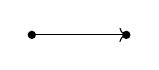
\begin{tikzpicture}[x=1cm,y=1cm]
 \fill (0,0) circle (1.5pt); \fill (1.2,0) circle (1.5pt);
 \draw[->] (0,0) -- (1.2,0);
\end{tikzpicture}
\end{adjustbox}
\end{center}
Зад. о классиф. отобр.
[Справа:] Инв. лишь $\dim\operatorname{Ker}$ и $\dim\operatorname{Coker}$.
Свод. к вложению.

\begin{center}
\begin{adjustbox}{max width=\linewidth}
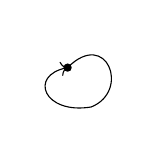
\begin{tikzpicture}[x=1cm,y=1cm]
 \fill (0,0) circle (1.5pt);
 \draw[->] (0,0) .. controls (0.5,0.5) and (0.8,-0.3) .. (0.3,-0.5)
 .. controls (-0.3,-0.6) and (-0.5,-0.1) .. (0,0);
\end{tikzpicture}
\end{adjustbox}
\end{center}
одно преобр.

\SourceFigure{GELFAND-P000464}{two-loop}{Один узел слева и две замкнутые дуги разного размера справа от него; у левого соединения видны стрелки, внешний верхний штрих бледен. Ниже начинается отдельная зачёркнутая строка.}
— зад. неразрешима (пара произв. лин. операторов).
[Перед «Она» зачёркнут короткий фрагмент:]
\Incomplete{GELFAND-P000464}{cancel-before-ona}{Короткий зачёркнутый фрагмент перед «Она» не восстановлен.}
Она свод. к зад. о коммутирующих
(\Unclear{GELFAND-P000464}{wild-name}{Гельф.} и Пономарёв).

[Зачёркнутая длинная строка; предположительное начало:]
\Unclear{GELFAND-P000464}{large-cancel-fragment}{Свод.}
\Incomplete{GELFAND-P000464}{large-cancel-remainder}{Остальная длинная зачёркнутая строка над «Пр-во и подпр-во» не восстановлена.}

\begin{equation*}
\left.
\begin{gathered}
\text{Пр-во и подпр-во.}\\
\text{Пр-во и }2\text{ подпр-ва}
\end{gathered}
\right\}\ \text{трив.}
\end{equation*}

\Unclear{GELFAND-P000464}{three-space-word}{Д-матая}: пр-во и [волнисто подчёркнуто:] $3$ лин. подпр-ва.

Инвариантов $9$, а не $8$!

\SourceFigure{GELFAND-P000464}{three-inward}{Три внешних узла — слева, снизу слева и снизу справа — соединены с верхним средним узлом; наконечники направлены к среднему узлу, правый соединён с густым пятном.}
(задача).

\SourceFigure{GELFAND-P000464}{four-inward}{На левом поле четырёхлучевая схема: четыре крайних узла по диагоналям и густой центральный узел; наконечники около центра, часть направлений закрыта чернилами.}

Пр-во и $4$ подпр-ва классиф. (Гельф. и Поном.) —
[зачёркнуто:] \Incomplete{GELFAND-P000464}{cancel-after-names}{Зачёркнутое слово после скобки с фамилиями не восстановлено.}
уже беск. число неразл.

\underline{Габриэль}: в каких графах конечное число неразл. систем?

Ответ: нарисовать схему Дынкина! — они и только они явл. такими графами.

Исключения: схемы с двойными (вообще кратными) стрелками.

\SourcePage{GELFAND-P000465}{unlabelled}
\underline{Теорема} (\Unclear{GELFAND-P000465}{theorem-names}{Ройтов или Назаровы}).
[Под первой фамилией вписано:] из Киева.
Опис. класс схем, где есть классифик. как у Гельф. и Пономарёва.

[Вся следующая строка волнисто подчёркнута:] Связь [зачёркнуто слово:]
\Incomplete{GELFAND-P000465}{cancel-specialities}{Зачёркнутое слово между «Связь» и «с особенностями» не восстановлено.}
с особенностями! — см. Артин, Тюрина, Брискорн.

[Прерывистая горизонтальная линия с точкой посередине.]

\underline{\underline{И.Б.}} [Волнисто подчёркнуто:] Категория вект. пр-в над точками и отобр. над стрелками.
(Граф фиксирован).
[Волнисто подчёркнуто:] Опред. прямой суммы. Это $\operatorname{Cat}(\Gamma)$ ($\Gamma$ — граф).
Морфизмы — отобр. над каждой точкой с коммут. диагр.

$\bullet$ Категория линейных пространств.

Важно: не обязательно \Unclear{GELFAND-P000465}{important-line}{отожд.} изоморфные.

Легко видно, что $\forall$ объект $=\sum$ неразлом. (однозн. с точн. до изом.).

$1)$ [Следующая строка волнисто подчёркнута:] Классиф. $\Gamma$, в к-рых конечное число неразл. объектов.

\underline{Огранич. связными:}

\SourceFigure{GELFAND-P000465}{dynkin-a-mark}{A с нижним n: горизонтальная цепь с тремя отмеченными вершинами слева, многоточием и одной отмеченной вершиной справа; рядом написано «(n точек)». Над третьей левой вершиной короткий поднятый косой штрих с верхним поперечным штрихом; его точная форма и значение не установлены.}

\SourceFigure{GELFAND-P000465}{dynkin-d}{D с нижним n: цепь с четырьмя отмеченными узлами слева, многоточием и правой развилкой с отмеченными диагональными концами. Между третьим и четвёртым левыми узлами есть небольшой направленный влево наконечник; точная связь слившихся штрихов наконечника и вершин остаётся неясной.}
$n\ge4$.

\begin{center}
\begin{adjustbox}{max width=\linewidth}
\begin{tikzpicture}[x=0.8cm,y=0.8cm]
 \node at (-0.7,0) {$E_k$}; \draw (0,0)--(4,0); \draw (1.6,0)--(1.6,-0.7);
 \fill (0,0) circle(1.5pt); \fill (0.8,0) circle(1.5pt);
 \fill (1.6,0) circle(1.5pt); \fill (2.4,0) circle(1.5pt);
 \fill (3.2,0) circle(1.5pt); \fill (4,0) circle(1.5pt);
 \fill (1.6,-0.7) circle(1.5pt);
\end{tikzpicture}
\end{adjustbox}
\end{center}
$k=6,7,8$ (слева обязательно $2$ отрезка).

Стрелки расставл. произвольно!!

$D_4$ — пр-во и $3$ подпр-ва.

Идея: нет циклов (напр. соб. значения), нет
\begin{center}
\begin{adjustbox}{max width=\linewidth}
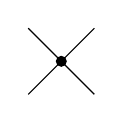
\begin{tikzpicture}[x=0.6cm,y=0.6cm]
 \draw (-0.7,0.7)--(0,0)--(0.7,0.7);
 \draw (-0.7,-0.7)--(0,0)--(0.7,-0.7);
 \fill (0,0) circle(2pt);
\end{tikzpicture}
\end{adjustbox}
\end{center}
— будет беск. число;
\begin{center}
\begin{adjustbox}{max width=\linewidth}
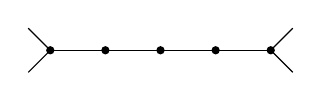
\begin{tikzpicture}[x=0.7cm,y=0.7cm]
 \draw (0,0)--(4,0);
 \draw (-0.4,0.4)--(0,0)--(-0.4,-0.4);
 \draw (4.4,0.4)--(4,0)--(4.4,-0.4);
 \fill (0,0) circle(1.5pt); \fill (1,0) circle(1.5pt);
 \fill (2,0) circle(1.5pt); \fill (3,0) circle(1.5pt); \fill (4,0) circle(1.5pt);
\end{tikzpicture}
\end{adjustbox}
\end{center}
тоже невозм., т.к. \Unclear{GELFAND-P000465}{fork-explanation}{отожд.}

$2)$ [Следующая строка волнисто подчёркнута:] Кол-во неразл. об. не зависит от напр. стрелок.

[Волнисто подчёркнуто:] Он характериз. набором размерностей!!

надо рассм. сист. корней.
$\gamma$ — полож. корень, $\alpha_i$ — пр. корни.
[Начальный глиф: \Unclear{GELFAND-P000465}{root-symbol}{$\gamma$}.]

Каждому корню — неразл. объект.
\begin{equation*}
 \gamma=\sum n_i\alpha_i,\qquad n_i\text{ — размерности!!}
\end{equation*}
[Глиф слева в предыдущей формуле: \Unclear{GELFAND-P000465}{root-symbol}{$\gamma$}.]
Кол-во = кол-ву \Unclear{GELFAND-P000465}{root-count}{простых} корней.

\begin{center}
\begin{adjustbox}{max width=\linewidth}
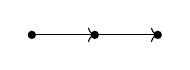
\begin{tikzpicture}[x=0.8cm,y=0.8cm]
 \draw[->] (0,0)--(1,0); \draw[->] (1,0)--(2,0);
 \fill (0,0) circle(1.5pt); \fill (1,0) circle(1.5pt); \fill (2,0) circle(1.5pt);
\end{tikzpicture}
\end{adjustbox}
\end{center}
\begin{equation*}
 \begin{array}{ccc}
 1&0&0\\
 0&1&0\\
 0&0&1\\
 1&1&0\\
 0&1&1\\
 1&1&1
 \end{array}
\end{equation*}
[Во второй строке средняя единица — \Unclear{GELFAND-P000465}{array-overwrite}{$1$} — написана поверх прежнего знака; справа сохранилась петля, похожая на часть нуля.]

\SourcePage{GELFAND-P000466}{unlabelled}
$3)$ [Следующая строка волнисто подчёркнута:] Рассм. те $\Gamma$, для к-рых $\operatorname{Cat}(\Gamma)$ разрешима.

\begin{center}
\begin{adjustbox}{max width=\linewidth}
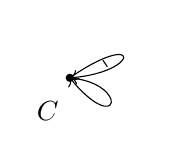
\begin{tikzpicture}[x=0.7cm,y=0.7cm]
 \fill (0,0) circle(1.5pt); \node at (-0.4,-0.6) {$C$};
 \draw[->] (0,0) .. controls (1.3,0.9) and (1.3,0.1) .. (0,0);
 \draw (0.60,0.32)--(0.68,0.20);
 \draw[->] (0,0) .. controls (1.1,-0.1) and (0.9,-1.1) .. (0,0);
\end{tikzpicture}
\end{adjustbox}
\end{center}
[Внутри верхней петли отдельный короткий косой штрих.]
Неразрешим. катег. — если есть влож. $C\to\operatorname{Cat}(\Gamma)$,
перев. неизом. объекты в неизом.

Они классиф. и соотв. расшир. схемам Дынкина!

\begin{center}
\begin{adjustbox}{max width=\linewidth}
\begin{tikzpicture}[x=0.7cm,y=0.7cm]
 \fill (0,0) circle(1.5pt);
 \draw[->] (0,0)--(0,1); \draw[->] (0,0)--(1,0); \draw[->] (0,0)--(-0.7,-0.9);
\end{tikzpicture}
\end{adjustbox}
\qquad
\begin{adjustbox}{max width=\linewidth}
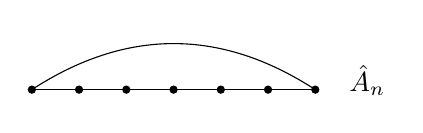
\begin{tikzpicture}[x=0.6cm,y=0.6cm]
 \draw (0,0)--(6,0); \draw (0,0) .. controls (2,1.3) and (4,1.3) .. (6,0);
 \fill (0,0) circle(1.5pt); \fill (1,0) circle(1.5pt); \fill (2,0) circle(1.5pt);
 \fill (3,0) circle(1.5pt); \fill (4,0) circle(1.5pt); \fill (5,0) circle(1.5pt);
 \fill (6,0) circle(1.5pt); \node at (7.1,0.2) {$\hat A_n$};
\end{tikzpicture}
\end{adjustbox}

\begin{adjustbox}{max width=\linewidth}
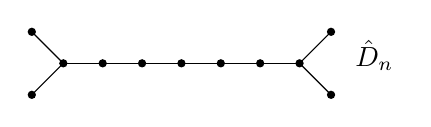
\begin{tikzpicture}[x=0.5cm,y=0.5cm]
 \draw (0,0)--(6,0);
 \draw (-0.8,0.8)--(0,0)--(-0.8,-0.8);
 \draw (6.8,0.8)--(6,0)--(6.8,-0.8);
 \fill (-0.8,0.8) circle(1.5pt); \fill (-0.8,-0.8) circle(1.5pt);
 \fill (0,0) circle(1.5pt); \fill (1,0) circle(1.5pt); \fill (2,0) circle(1.5pt);
 \fill (3,0) circle(1.5pt); \fill (4,0) circle(1.5pt); \fill (5,0) circle(1.5pt);
 \fill (6,0) circle(1.5pt); \fill (6.8,0.8) circle(1.5pt); \fill (6.8,-0.8) circle(1.5pt);
 \node at (7.9,0.2) {$\hat D_n$};
\end{tikzpicture}
\end{adjustbox}
\qquad
\begin{adjustbox}{max width=\linewidth}
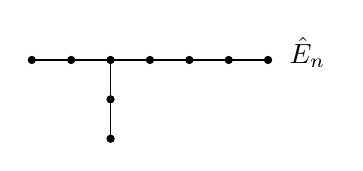
\begin{tikzpicture}[x=0.5cm,y=0.5cm]
 \draw (0,0)--(6,0); \draw (2,0)--(2,-2);
 \fill (0,0) circle(1.5pt); \fill (1,0) circle(1.5pt); \fill (2,0) circle(1.5pt);
 \fill (3,0) circle(1.5pt); \fill (4,0) circle(1.5pt); \fill (5,0) circle(1.5pt);
 \fill (6,0) circle(1.5pt); \fill (2,-1) circle(1.5pt); \fill (2,-2) circle(1.5pt);
 \node at (7,0.2) {$\hat E_n$};
\end{tikzpicture}
\end{adjustbox}
\end{center}

(появл. в теории [Над строкой перед «групп» зачёркнута короткая запись: \Unclear{GELFAND-P000466}{cancel-in-group-comment}{гр}.] групп,
порождённых отражениями.)

Это все графы, для к-рых зад. разрешима.

\underline{\underline{В. Бухштабер.}}

[Следующая строка дважды подчёркнута:] Теор. \Unclear{GELFAND-P000466}{theorem-name}{Лазура}.
$\Lambda=\mathbb Z[a_1,\ldots,a_n,\ldots]$, $\operatorname{deg}a_n=n\ge1$.

\underline{Док-во.}
\Unclear{GELFAND-P000466}{decomposables-quotient}{$\Lambda\to\bar\Lambda=\Lambda/(\text{разл.})$}.

$\bar\Lambda$ — универс. кольцо для [вписано в пузыре: таких] полиномов $h(x,y)$,
[Слова «универс. кольцо для полиномов» волнисто подчёркнуты.]
[вписано в пузыре: что] $h(x,y)=h(y,x)$, $h(x,0)=0$,
\begin{equation*}
 h(y,z)+h(x,y+z)=h(x,z)+h(y,x+z).
\end{equation*}
Это когомологии: $dh=0$ [Под «dh»: (\Unclear{GELFAND-P000466}{cycle-caption}{циклы})] (в бар-конструкции для полиномов).
\begin{center}
\Unclear{GELFAND-P000466}{cohomology-conventions}{$\operatorname{Ext}^{*,*}_{A[x]}(A,A)=H^{*,*}(A[x])$}.
\end{center}
$A[x]\to A[x]\otimes\bar A[y]$, \Unclear{GELFAND-P000466}{normalized-coproduct}{$x\to x+y$}.

Когом. счит. с пом. резольвент.
Бар-констр. — одна из резольвент.
\begin{equation*}
 \mathcal A:\quad A[x]\overset{\Delta}{\longrightarrow}A[x]\otimes\bar A[y]
 \longrightarrow A[x]\otimes\bar A[y]\otimes\bar A[z]\longrightarrow\ldots
\end{equation*}
$\bar A[y]$ — многочлены без своб. члена.

Получ. ацикличный комплекс, к-рый прим. для вычисл. когомологий
(ставим всюду [Ниже «всюду» приписано: $h(x,y)$.] —
$\tilde a\Rightarrow a\otimes1+1\otimes a)=\Delta a)$.
[Левая запись предыдущей формулы: \Unclear{GELFAND-P000466}{primitive-condition}{$\tilde a\Rightarrow$}. Обе исходные закрывающие скобки сохранены.]

Надо классиф. циклы в конкретной резольвенте.
\begin{center}
\Unclear{GELFAND-P000466}{cohomology-conventions}{$0\longrightarrow B\longrightarrow Z\longrightarrow H^2(A[x])\longrightarrow0$}.
\end{center}
$x^n\to(x+y)^n-x^n-y^n$ (это границы).

\SourcePage{GELFAND-P000467}{unlabelled}
Переход к \Unclear{GELFAND-P000467}{opening-word}{полученн.} резольв. с пом. функтора $\operatorname{Hom}(\cdot,A)$

В ациклич. резольв.
\begin{gather*}
 x\longrightarrow x+y\\
 x^n\longrightarrow(x+y)^n.
\end{gather*}

Надо рассм. \Unclear{GELFAND-P000467}{hom-module-conventions}{$\operatorname{Hom}_{A[x]}(\mathcal A,A)$}
(по $1$-му сомножителю \Unclear{GELFAND-P000467}{parenthetical-abbreviation}{уст.} структ. $A[x]$-мод.).
\begin{center}
\Unclear{GELFAND-P000467}{cochain-conventions}{$A\overset d\longrightarrow A[y]\overset d\longrightarrow A[y]\otimes A[z]\overset d\longrightarrow\ldots$}
\end{center}
\begin{center}
\Unclear{GELFAND-P000467}{cochain-conventions}{$\Delta\longrightarrow d:\quad x^n\longrightarrow(x+y)^n-x^n-y^n$}
\end{center}
\begin{center}
\Unclear{GELFAND-P000467}{cochain-sign}{$\Delta:\quad h(x,y)\longrightarrow h(\underset{\substack{\Vert\\x+z}}{\Delta x},y)-h(x,\underset{\substack{\Vert\\y+z}}{\Delta y})$}
\end{center}
[Знак между двумя членами справа густо наведён.]

$\mathcal A$ — послед. $A[x]$-модулей\Unclear{GELFAND-P000467}{module-ending-punctuation}{,}

$A[x]\otimes y^k$ — подмодули
[Слово «подмодули» волнисто подчёркнуто.]

Из-за $\overline{A[y]}$:
$x^n\longrightarrow(x+y)^n-x^n$ (т.к. без своб. члена)

[По правому полю длинная вертикальная черта, заканчивающаяся немного ниже разделителя.]
[Под текстом разделитель: два горизонтальных отрезка с точкой между ними; нижняя часть кадра пустая.]

\SourcePage{GELFAND-P000468}{unlabelled}
\underline{13/$\overline{\underline{\mathrm{XI}}}$–72г.}\quad \underline{Сем. Гельфанда.}

\underline{Л. Вассерштейн.}

$\underline{\underline{A}}$ — ассоциат. кольцо (не обязательно с $1$).

$\underline{\underline{iA}}$ — кольцо с формально присоед. единицей.

$iA/A=\mathbb Z$, $A$ — двустор. идеал в $iA$.

$GA$ — мульт. группа кольца.
$GA\subset A$.

$(a,b)\to a+b+ab$. Это бинарная ассоц. опер.
[На правом поле перед формулой две вертикальные черты:]
$\Vert\ (e+a)(e+b)-e=a+b+ab$.

[Перед $GA$ зачёркнуто:]
\Unclear{GELFAND-P000468}{initial-cancel}{$iA$}.
$\underline{\underline{GA}}$ — мн-во обратимых элементов отн. этой операции.

$a\to1+a$, $A\to1+A$ гомоморфизм \underline{в обычные обрат. элем.}
[«гомоморфизм» волнисто подчёркнуто; «в обычные» и «обрат. элем.» подчёркнуты двумя отдельными строками.]

$f:A\to B$, \Unclear{GELFAND-P000468}{image-containment}{$f(GA)\subset GB$}.

$i,G$ — функторы в кат. колец с $1$ и кат. групп.

$\underline{\underline{M_kA}}$ — матрицы $k\times k$ с обычным умножением.

$\underline{\underline{\tilde\Omega A}}=\{a=(a_{ij})\}$, в $\forall$ строке и столбце конеч. число элем. $\ne0$.
(это кольцо).

$\underline{\underline{MA}}$ — подкольцо конечных матриц (конечное число элем. $\ne0$).
(двустор. идеал в $\tilde\Omega A$).

$\underline{\underline{\Omega A}}=\tilde\Omega A/MA$.
[Буква перед $A$ слева густо наведена.]

$M,\tilde\Omega,\Omega$ — функторы.

$\underline{\underline{\Theta A}}\subset MA$ — \Unclear{GELFAND-P000468}{triangular-convention}{верхние треугольные} $a=(a_{ij})$:
$a_{ij}=0$ при $i\le j$
[Под двойным подчёркиванием $\Theta A$ отдельная короткая вертикальная черта; после неравенства густо зачёркнуты расположенные друг под другом знаки:]
\Unclear{GELFAND-P000468}{cancel-inequality}{знаки}.

\underline{Замечание}. Если $N\overset{\sim}{\longrightarrow}N$ биекция, то есть отобр. кольца матриц
([зачёркнуто:] \Unclear{GELFAND-P000468}{cancel-auto}{эт}
автом.) — перестан. одноврем. строк и столбцов.
(\Unclear{GELFAND-P000468}{inner-ambient}{внутр. автом.} перестан. строк и столбцов).

\Unclear{GELFAND-P000468}{next-word}{Даже} если $N\to N$ любое отобр., то ему соот. \Unclear{GELFAND-P000468}{arbitrary-reindexing}{\underline{эндоморфизм}}.

$GMA$ — мульт. группа $MA$, $GMA\subset MA$.

Симплициальная структура в $MA$.
[Заголовок волнисто подчёркнут.]

$X\subset GMA$ наз. симплексом; если \Unclear{GELFAND-P000468}{left-shift-convention}{левым сдвигом} и сопряжением матрицей перестановок
его можно перевести в $\Theta A$.

Заметим, что $G\Theta A=\Theta A$ как множество (они \Unclear{GELFAND-P000468}{final-word}{нильпотентны}).

[По правому краю кадра тонкая прерывистая вертикальная линия; внизу справа чёрный прямоугольник.]
\SourcePage{GELFAND-P000469}{unlabelled}
[Зачёркнутый знак перед первой строкой: \Unclear{GELFAND-P000469}{top-cancelled}{неразборчиво}.]
На самом деле \underline{$GMA\supset\Theta A$}.

\underline{Отметим вершину: $0$} --- единица группы $GMA$.

\underline{$SA$} --- соответствующая симплициальная схема.

(Историч. замечание: Володин использовал $SA$ для опр. функторов
\Unclear{GELFAND-P000469}{top-functor-index}{$K_{\mathbb C}^{n}$})
[Под строкой: по существу.]

\medskip
Пусть в кольце $A$ есть единица. Тогда положим
\begin{equation*}
K_nA=\pi_{n-1}SA,\qquad n\geq1.
\end{equation*}
При $n\geq2$ там есть структура группы, коммутативной при $n\geq3$.

\underline{Другое опред. групповой структуры (коммутативной).}

\underline{Лемма Уайтхеда}

Рассм. сфероид $s\colon Z^n\longrightarrow SA$.
На $SA$ действует группа подстановок $f\colon N\longrightarrow N$.
Получ. новый сфероид $s^f$:
\begin{center}
\begin{adjustbox}{max width=\linewidth}
\begin{tikzcd}
Z^n \arrow[rr] \arrow[dr,"s^f"'] & & SA \arrow[dl,"f"] \\
& SA &
\end{tikzcd}
\end{adjustbox}
\end{center}
Они всегда гомотопны.

\underline{Идея док-ва:}

$\operatorname{Im}s\subset M_kA$.
\Unclear{GELFAND-P000469}{middle-block-argument}{$s=\begin{pmatrix}sz&0\\0&0\end{pmatrix}$}.

Всё сводится к случаю
\begin{equation*}
s^f=\begin{pmatrix}0&0\\0&sz\end{pmatrix}.
\end{equation*}
[В обеих матрицах проведены горизонтальная и вертикальная разделительные черты.]

($f$ специального вида: $fi=i+k$, на $\infty$ подправляем).

\begin{equation*}
\begin{pmatrix}a&0\\0&0\end{pmatrix}\qquad
\begin{pmatrix}a&a\\0&0\end{pmatrix}\qquad
\begin{pmatrix}0&a\\-1&0\end{pmatrix}\qquad
\begin{pmatrix}0&0\\-1&a\end{pmatrix}\qquad
\begin{pmatrix}0&0\\0&a\end{pmatrix}
\end{equation*}
Это 5 сфероидов. Это гомотопия. Каждые 2 соседних элементарно гомотопны:
\begin{equation*}
s_1,s_2\colon S\longrightarrow S'
\end{equation*}
наз. элем. гомотопными, если $\forall$ симплекса $X\subset S$, $s_1X\cup s_2X$
есть симплекс в $S'$.

Пусть все $a$ лежат в одном симплексе $X$.
Тогда $\begin{pmatrix}a&0\\0&0\end{pmatrix}$ и
$\begin{pmatrix}a&a\\0&0\end{pmatrix}$ лежат в одном симплексе.

Пусть $a_0^{-1}\in X$. Умножим на $a_0$. Тогда они станут верхнетреуг.
Если все $a$ верхне-треугольные, то все 5 матриц лежат в одном симплексе.

\medskip
\underline{Структура коммут. группы в $K_nA$.}
\begin{equation*}
MA\times MA\overset{\oplus}{\longrightarrow}MA
\end{equation*}
\begin{equation*}
fi=2i,\qquad gi=2i+1,\qquad f,g\colon\mathbb N\longrightarrow\mathbb N,
\qquad a\oplus b=a^f+b^g.
\end{equation*}
[Справа, за вертикальной чертой: некоммут., неассоц., без нейтр. элем.]

[У нижнего левого края, вне основной области текста:
\Unclear{GELFAND-P000469}{margin-left-bottom}{отдельный наклонный штрих и знак, похожий на закрывающую скобку}.]

\SourcePage{GELFAND-P000470}{unlabelled}
она индуцирует отобр. $SA\times SA\longrightarrow SA$,
что даёт операции на всех $K_i$, $i\geq0$. (корр. прв. по лемме Уайтхеда)
Они коммутативны и совпад. с ранее введёнными в силу взаимной
дистрибутивности, проверяемой по лемме Уайтхеда.

\medskip
Можно определить сумму --- $H$-пр-во.
На $\widetilde{\Omega}A$ склад. даже беск. число матриц!
Отсюда оно будет иметь тривиальные $K$-функторы.

\medskip
\underline{$K_1A=\pi_0SA$.}

Это мн-во компон. связности в $GMA$.

$EA$ --- связная компон. единицы. (произведения элем. матриц),
[вставлено под строкой к слову «элем.»: псевдотреугольные]
\begin{equation*}
\fbox{$\begin{gathered}A\ni1\\\text{или}\\AA=A\quad\text{(в кольцевом умн.)}\end{gathered}$}
\quad\Longrightarrow\quad EA=[GMA,GMA]=[EA,EA].
\end{equation*}

$K_2A$ --- гомот. классы петель. Петли --- соотношения элем. матриц.

$\Theta A$ имеет образующие $a^{ij}$
[далее зачёркнуто: \Incomplete{GELFAND-P000470}{middle-generator-cancelled}{Выражение после $a^{ij}$ полностью перекрыто многократным зачёркиванием; внутреннее содержание не прочитано.}]
(на $i,j$-м месте стоит $a\in A$).
[Под словом «Петли» короткая стрелка вниз-влево, к области зачёркнутой записи.]

Соотнош.: Стейнберга
\begin{gather*}
a^{ij}\ast b^{ij}=(a+b)^{ij},\\
[a^{ij},b^{jk}]=(ab)^{ik}
\end{gather*}
и у нек-рых коммутатор $0$.

Это определяющие соотношения.

Пусть $StA$ --- группа, порожд. этими образ. и соотн.
\begin{equation*}
0\longrightarrow K_2A\longrightarrow StA\longrightarrow EA\longrightarrow0
\end{equation*}
[Под $StA$, с соединительным штрихом: гомот. классы путей из $0$ куда-то
(с фикс. нач. и концом).]

\medskip
[Слева от следующей формулы: \Unclear{GELFAND-P000470}{lower-margin-mark}{неразборчивый одиночный знак}.]
\begin{equation*}
K_2A=H_2EA\qquad\sim\qquad
StA=\text{универс. центр. расширение }EA.
\end{equation*}
[Под $H_2EA$: (гомологии группы).]

\underline{Задача:} пусть есть 3 матрицы в $GMA$. Все отрезки --- симплекс.
Тогда все 3 --- симплекс.

Обобщение: если любая пара симплекс, то все симплекс.
(пр-во \underline{толерантности})

\medskip
\underline{Д. А. Каждан.}\qquad\underline{Производная категория.}

$C$ --- абелева категория. Рассм. категорию комплексов $K_C$.

\begin{center}
\begin{adjustbox}{max width=\linewidth}
\begin{tikzcd}
\vdots & \vdots \\
K_n \arrow[u] \arrow[r] & K'_n \arrow[u] \\
K_{n-1} \arrow[u] \arrow[r] & K'_{n-1} \arrow[u] \\
\vdots \arrow[u] & \vdots \arrow[u]
\end{tikzcd}
\end{adjustbox}
\end{center}
[Справа от схемы, зачёркнуто:
\Unclear{GELFAND-P000470}{bottom-cancelled-words}{сост. об.}.]
\underline{морфизмы $f$ --- гомот. классы морфизмов комплексов.}
[После слова «морфизмов» зачёркнут знак:
\Unclear{GELFAND-P000470}{bottom-right-cancelled}{неразборчиво}.]

\begin{equation*}
S\subset\operatorname{Hom}K_C
\end{equation*}
[Под $S$, с соединительным штрихом: морф., индуц. изоморфизм гомологий.]

\SourcePage{GELFAND-P000471}{unlabelled}
\underline{Лемма.} Пусть $f,g\colon K\longrightarrow K'$ два морфизма.

След. утв. эквивалентны:

$1^{\circ}$. $\exists K_1$, $s_1\in S$:
\begin{center}
\begin{adjustbox}{max width=\linewidth}
\begin{tikzcd}
K_1 \arrow[r,"s_1"] & K \arrow[r,shift left,"f"] \arrow[r,shift right,"g"'] & K'
\end{tikzcd}
\end{adjustbox}
\end{center}
\begin{equation*}fs_1=gs_1.\end{equation*}

$2^{\circ}$. $\exists K_2$, $s_2\in S$
\begin{center}
\begin{adjustbox}{max width=\linewidth}
\begin{tikzcd}
K \arrow[r,shift left,"f"] \arrow[r,shift right,"g"'] & K' \arrow[r,"s_2"] & K_2
\end{tikzcd}
\end{adjustbox}
\end{center}
\begin{equation*}s_2f=s_2g.\end{equation*}

\medskip
$L_C$ --- те же объекты, а морфизмы: разреш. обращать $s^{-1}$ и
[вставлено под строкой: соотношения Оре.]
Лемма даёт возможно корректно опр. произведение.

\medskip
[Над «См.»: \Unclear{GELFAND-P000471}{middle-reference-mark}{крестообразная помета}.]
См. \underline{Hartshorne.} Residues and duality.

\medskip
\underline{В. Бухштабер.}

Ссылки:\quad К.-Э.\quad 213--223\quad (Картан и Эйленберг)

\hspace{2em}М.\quad 358--370\quad (\Unclear{GELFAND-P000471}{middle-maclane}{Маклейн})

\hspace{2em}Адамс\quad Мат.\quad $3\colon4$\quad стр. 7--19.

\medskip
\begin{equation*}
A=\sum_{n\geq0}A_n\qquad\text{--- градуир. кольцо.}
\end{equation*}
$A_n$ --- $A_0$-модуль для любого $n\geq0$.
\begin{equation*}
0\longleftarrow A_0\overset{\varepsilon}{\longleftarrow}A
\longleftarrow C_1\longleftarrow C_2\longleftarrow\cdots
\longleftarrow C_s\overset{d_{s+1}}{\longleftarrow}C_{s+1}
\longleftarrow\cdots
\end{equation*}
($\varepsilon$ сопост. \Unclear{GELFAND-P000471}{lower-augmentation-a}{$A$}
нулев. компон. каждому $a\in A$).

Доп. до \underline{градуир. своб. резольвенты.}

Функтор \Unclear{GELFAND-P000471}{lower-hom-coefficient}{$\operatorname{Hom}_A(\cdot,A)$}
переводит $d_s$ в $(d_s)^*$.
\begin{equation*}
H^s(A)=\ker(d_{s+1})^*/\operatorname{Im}(d_s)^*
\end{equation*}

\underline{Теорема:}\quad 1) Сущ. своб. резольвента

\hspace{6em}2) Группы $H^s(A)$ не зависят от резольвенты.

\begin{equation*}
H(A)=\sum_{s=0}^{\infty}H^s(A)\qquad\text{--- градуированное кольцо.}
\end{equation*}
Будет дано опр. умн. \underline{Йонеда.}
\begin{gather*}
f\in H^i(A),\quad g\in H^j(A),\quad fg\in H^{i+j}(A),\\
\widetilde f\colon C_i\longrightarrow A_0;\qquad
\widetilde g\colon C_j\longrightarrow A_0.
\end{gather*}

\SourcePage{GELFAND-P000472}{unlabelled}
\SourceFigure{GELFAND-P000472}{top-product-diagram}{Схема вверху слева.
Верхний ряд: $C_i\longleftarrow\cdots\quad\cdots\quad C_{i+j}$.
Нижний ряд: $A_0\longleftarrow A\longleftarrow C_1\longleftarrow\cdots\longleftarrow C_j$;
буква в узле $C_1$ густо обведена. От $C_i$ к левому $A_0$ идёт сплошная
наклонная стрелка с подписью $\widetilde f$, от $C_i$ к $A$ --- прерывистая
стрелка вниз. От $C_{i+j}$ к $C_j$ идёт наклонная стрелка с разрывом стержня.
Под $C_j$ --- стрелка $\widetilde g$ вниз к ещё одному $A_0$.
Начертание обведённого узла и характер разрыва правой стрелки требуют сверки с оригиналом.}

Получим гомоморфизм $C_{i+j}\longrightarrow A_0$.

Получится
\begin{equation*}
A\underset{\text{сопост.}}{\rightsquigarrow}H(A)\qquad\text{(кольцо)}
\end{equation*}
$H(A)$ вообще говоря некоммутативно (!) по настоящему.
На этом основана классифик. многозн. групп
(В топологии до сих пор встр. только коммут. кольца --- там всегда алгебры Хопфа).

\underline{Станд. резольвента или $B$-резольвента.}
\begin{equation*}
\overline A=\sum_{n>0}A_n
\end{equation*}
\begin{equation*}
C_1=A\otimes_{A_0}\overline A\qquad\text{В дальнейшем }A_0\text{ опускается}
\end{equation*}
(Исх. кольца коммутативны!)
\begin{gather*}
C_s=A\otimes(\overline A)^s.\\
d_{s+1}\colon A\otimes(\overline A)^{s+1}\longrightarrow A\otimes(\overline A)^s
\end{gather*}
\begin{multline*}
d_s\bigl(a_0[a_1|a_2|\ldots|a_s]\bigr)
=(-1)^{\varepsilon(0)}a_0a_1[a_2|\ldots a_s]\\
+\sum(-1)^{\varepsilon(n)}a_0[a_1|\ldots|a_na_{n+1}|\ldots a_s]
\end{multline*}
$\varepsilon(n)$ --- некоторые ф-ии от номера,
[зачёркнуто: Для чётной градуир. $\varepsilon(n)=n$.]
[Вписано ниже: $\varepsilon(n)=n$, если все элем. чётные.]

\begin{equation*}
\operatorname{Hom}_A(C_s,A_0)\simeq(\overline A^*)^s,
\qquad\overline A^*=\operatorname{Hom}_{A_0}(\overline A,A_0)
\end{equation*}
\begin{equation*}
d_s^*\colon[\alpha_1|\alpha_2|\ldots|\alpha_{s-1}]
=\sum(-1)^{\varepsilon(n)}
[\alpha_1|\ldots|\overline\Delta\alpha_n|\ldots|\alpha_{s-1}].
\end{equation*}
\begin{equation*}
\varepsilon(n)=n,\quad\text{если }\operatorname{deg}\alpha_i=2k_i
\end{equation*}

\underline{Опред. $\overline\Delta$.}
\SourceFigure{GELFAND-P000472}{lower-coproduct-box}{В фигурной рамке три строки.
Верхняя: $A\otimes_{A_0}A$ слева, $A$ справа; между ними толстая стрелка
с явным правым остриём и левым концом, также похожим на остриё;
под стрелкой $\mu$ (умн.). Вторая: $A^*\otimes_{A_0}A^*\longleftarrow A^*\colon\Delta$,
под $\Delta$: двойств. к $\mu$. Третья:
$a\otimes1+1\otimes a+\overline\Delta a\longleftarrow a$,
справа (опред. $\overline\Delta$). Направленность верхней стрелки не восстановлена по математическому ожиданию.}

На самом деле
\Unclear{GELFAND-P000472}{lower-reduced-image}{$\operatorname{Im}\overline\Delta\subset\overline{A^*}$}.

Отсюда ещё одно определение умножения.
\begin{equation*}
C_s^*\qquad f=[\alpha_1|\ldots|\alpha_s]
\end{equation*}
$C_{s'}^*$\quad
\Unclear{GELFAND-P000472}{bottom-prime-index}{$g=[\alpha'_1|\ldots|\alpha'_{s'}]$;
\quad $f\cdot g=[\alpha_1|\ldots|\alpha_s|\alpha'_1|\ldots|\alpha'_{s'}]$.}

\SourcePage{GELFAND-P000473}{unlabelled}
\underline{20/XI--72. Сем. Гельфанда.}

\underline{Костюченко.}\qquad\underline{Один пример.}
\begin{gather*}
v''+2a\lambda v'+b\lambda^2v=0,\\
v(0)=v(\pi)=0.
\end{gather*}
в $L_2[0,\pi]$.

[Справа вверху, формула с нижней рамочной чертой:]
\begin{equation*}
\frac{\partial^2u}{\partial x^2}
+2a\frac{\partial^2u}{\partial x\partial t}
+b\frac{\partial^2u}{\partial t^2}=0,\qquad 0<x<\pi,
\end{equation*}
\Unclear{GELFAND-P000473}{top-time-inequality}{$0\leq t<+\infty$}.
\underline{Пучок эллипт. ур-я.}

\underline{$a^2<b$};\qquad\underline{$b>0$}.
\begin{equation*}
v_k(x)=e^{\gamma kx}\sin kx,\qquad
\underline{\gamma=\frac{-a}{\sqrt{b-a^2}}},\qquad k=\pm1,\ \pm2,\ldots
\end{equation*}

1. Система полна, но неизв., как находить коэффициенты.
Это вопрос о нахожд. биортог.
\Unclear{GELFAND-P000473}{upper-system-correction}{системы. [Окончание обведено; после точки отдельный зачёркнутый знак.]}
(нах. в терминах обр. ф-и к интегр. Кристоффеля--Шварца)

(\underline{биортог. система есть})

2. \underline{Это не базис!} (не любой вектор разл. в сход. ряд по этой сист.)

[Зачёркнуто: \Unclear{GELFAND-P000473}{middle-cancelled-even}{Даже}.]
\underline{Более того:} если есть разл. в $L^2$, то предел --- аналит.
ф-я! --- и вып. беск. число краев. условий (верно и обратное).

Нельзя суммировать методом Абеля 1-го порядка.
\underline{если}
\Unclear{GELFAND-P000473}{middle-abel-coefficient}{$\displaystyle\sum_{\lambda_k>0}e_k e^{\lambda_kt}v_k(x)$}
[зачёркнуто: \Incomplete{GELFAND-P000473}{middle-abel-cancelled}{Два коротких фрагмента после $v_k(x)$ перекрыты зачёркиванием; их содержание не прочитано.}]
им. предел при $t\to0$,
то \underline{ф-я предельная} аналитична.

(Дискредитация метода Фурье для эллипт. ур-я)

При нек-рых неразд. условиях можно решать.

[Перед следующей строкой две зачёркнутые пометы:
\Unclear{GELFAND-P000473}{lower-cancelled-marks}{неразборчиво}.]
\underline{Причина плохого повед.:} резольвента $\exp$ растёт в углах
\begin{center}
\begin{adjustbox}{max width=\linewidth}
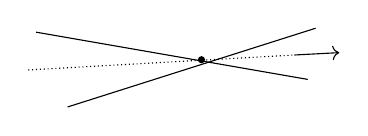
\begin{tikzpicture}
\draw (-2.1,0.35) -- (1.35,-0.25);
\draw (-1.7,-0.6) -- (1.45,0.4);
\draw[densely dotted] (-2.2,-0.13) -- (1.18,0.06);
\draw[->] (1.18,0.06) -- (1.75,0.09);
\fill (0,0) circle (1.3pt);
\end{tikzpicture}
\end{adjustbox}
\end{center}

На $[0,\pi-\varepsilon]$ переопределена.

На $[0,\pi+\varepsilon]$, $0<\varepsilon<\pi$ она остаётся полной !!! (И. Бернштейн)

На $[0,2\pi]$ возникает много ортог. ф-ий.

\underline{Задача теории целых ф-ий.}
\begin{equation*}
\int_0^\pi f(x)e^{\gamma kx}\sin kx\,dx=0
\quad\Longrightarrow\quad
F(\lambda)=\int_0^\pi f(x)e^{\gamma\lambda x}\sin\lambda x\,dx
\end{equation*}
$F(\lambda)$ целая ф-я $\exp$ типа. Она $0$ в целых точках
$F(n)=0$, $n>0$.

\underline{Надо учесть специфику.}

На $[0,\pi-\varepsilon]$ срабатывает тип и индик. диаграмма.

Единственность --- ?

Неизвестно, что будет, если заменить $k$ на $\lambda_k$.

\SourcePage{GELFAND-P000474}{unlabelled}
\underline{И. М. Гельфанд}\qquad\underline{о раб. Арнольда.}
\begin{equation*}
(\mathbb R^n,0)\longrightarrow(\mathbb R,0)
\end{equation*}
$f(x)=0$ --- гиперпов.

Как ведёт себя гиперпов. в окр. $0$ --- ?

$f\in C^{\infty}$;\quad $f(0)=0$, $df(0)=0$. (крит. точка).

(На самом деле рассм. $\mathbb C^n\longrightarrow\mathbb C$)

Эквив. гиперпов. --- отлич. заменой переменных
\begin{equation*}
(\mathbb R^n,0)\longrightarrow(\mathbb R^n,0)\qquad\text{(диффеом.)}.
\end{equation*}

\underline{Простая гиперпов.:}\qquad\underline{$f(x)=0$}

если пошевелить, то будет конечное число орбит
в струях пор. $N$ (оценка числа орбит не зависит от номера $N$).

Перечисление простых орбит:
\begin{center}
\begin{adjustbox}{max width=\linewidth}
\begin{tikzpicture}[x=0.65cm,y=0.7cm]
\node[circle,draw,inner sep=1.5pt] (a0) at (0,0) {};
\node[circle,draw,inner sep=1.5pt] (a1) at (0.8,0) {};
\node[circle,draw,inner sep=1.5pt] (a2) at (1.6,0) {};
\node[circle,draw,inner sep=1.5pt] (a3) at (2.3,0) {};
\node[circle,draw,inner sep=1.5pt] (a4) at (5,0) {};
\draw (a0)--(a1)--(a2)--(a3)--(2.9,0);
\node at (3.55,0) {$\cdots$};
\draw (4.3,0)--(a4);
\node[circle,draw,inner sep=1.5pt] (d0) at (0,-1) {};
\node[circle,draw,inner sep=1.5pt] (d1) at (0.8,-1) {};
\node[circle,draw,inner sep=1.5pt] (d2) at (4.9,-1) {};
\node[circle,draw,inner sep=1.5pt] (d3) at (5.5,-0.55) {};
\node[circle,draw,inner sep=1.5pt] (d4) at (5.5,-1.45) {};
\draw (d0)--(d1)--(1.5,-1);
\node at (2.35,-1) {$\cdots$};
\draw (4,-1)--(d2)--(d3);
\draw (d2)--(d4);
\node[circle,draw,inner sep=1.5pt] (e0) at (6.7,0) {};
\node[circle,draw,inner sep=1.5pt] (e1) at (7.4,0) {};
\node[circle,draw,inner sep=1.5pt] (e2) at (8,0) {};
\node[circle,draw,inner sep=1.5pt] (e3) at (8.6,0) {};
\node[circle,draw,inner sep=1.5pt] (e4) at (9.2,0) {};
\node[circle,draw,inner sep=1.5pt] (e5) at (10.1,0) {};
\node[circle,draw,inner sep=1.5pt] (e6) at (11,0) {};
\node[circle,draw,inner sep=1.5pt] (e7) at (8,-0.65) {};
\draw (e0)--(e1)--(e2)--(e3)--(e4);
\draw (e2)--(e7);
\draw[dashed] (e4)--(e5)--(e6);
\node[right] at (11.6,-0.2) {$E_6,E_7\text{ и }E_8$};
\end{tikzpicture}
\end{adjustbox}
\end{center}

Далее: Большинство орбит простые
([зачёркнуто: \Unclear{GELFAND-P000474}{middle-parenthetic-cancelled}{неразборчивый короткий фрагмент}]
как правило, орбита-простая).
\underline{Непростые коразмерности 6.}

\Unclear{GELFAND-P000474}{middle-simple-equation}{$x_1^{n+1}+x_2^2+\cdots\,\ast=0$}
--- соотв. 1-му типу.

\underline{Версальная деформация.}
\begin{gather*}
F(x,\lambda)=0,\qquad F(x,0)=f(x),\\
\lambda=(\lambda_1,\lambda_2,\ldots,\lambda_k)
\end{gather*}
Всякая другая деф. эквив. деф., индуц. из этой след. образом:

\Unclear{GELFAND-P000474}{middle-induced-variables}{$G(y,\mu)=F(X(y,\mu),\Psi(\mu))$}
и $X(y,0)=y$, $\Psi(0)=0$.

\underline{Правило построения верс. сем-ва:}

Берём орбиту и мн-ие, трансверс. к орбите
\begin{center}
\begin{adjustbox}{max width=\linewidth}
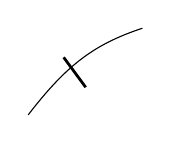
\begin{tikzpicture}
\draw (-0.7,-0.55) .. controls (-0.2,0.1) and (0.15,0.35) .. (0.75,0.55);
\draw[line width=1pt] (-0.25,0.18)--(0.03,-0.2);
\end{tikzpicture}
\end{adjustbox}
\end{center}

\Unclear{GELFAND-P000474}{lower-taylor-coefficient}{$\displaystyle
F(x,\lambda)=f(x)+\sum a_i\left.\frac{\partial F}{\partial\lambda_i}\right|_{\lambda_i=0}
=f(x)+\sum c_i\varphi_i(x)+O(\lambda^2)$.}

\underline{\Unclear{GELFAND-P000474}{lower-definition-heading}{Опред. Инфинитезимальную версальную деформацию:}}
если $\forall$ ф-я $a(x)$ предс. в виде
\begin{equation*}
a(x)=\sum\frac{\partial f}{\partial x_i}\cdot h_i(x)+\sum_{i=1}^{k}c_i\varphi_i(x)
\end{equation*}
$a(x)$ задаёт инфинитезим. верс. деформ.

($\varphi_i$ порожд. лок. кольцо глад отобр.)

[Зачёркнутая запись, начинающаяся открывающей скобкой:
\Incomplete{GELFAND-P000474}{bottom-cancelled-taylor}{Слово или короткая фраза перед «из разл. по Тейлору» перекрыта несколькими чертами и не прочитана.}]
(из разл. по Тейлору той ф-ии)

Важно: факторкольцо по \underline{якобиеву идеалу}
$\left(\left\{\dfrac{\partial f}{\partial x_i}\right\}\right)$.

\underline{Фактор} --- конечномерное пр-во размерности $k$.

\SourcePage{GELFAND-P000475}{unlabelled}
\underline{\underline{$f=z_1^{k+1}+z_2^2+\cdots+z_n^2$.}}

Тогда
\Unclear{GELFAND-P000475}{top-derivatives}{$\displaystyle
\frac{\partial f}{\partial z_1}=z_1^k,\quad
\frac{\partial f}{\partial z_2}=z_2,\ldots$},

отсюда факторкольцо --- пр-во размерности $k$.

\Unclear{GELFAND-P000475}{top-phi-indices}{$\varphi_i=1,z_i,z_i^2,\ldots,z_1^{k-1}$.}

Верс. деформация:
\begin{equation*}
\underline{\lambda_0+\lambda_1z_1+\cdots+\lambda_{k-1}z_1^{k-1}+z_1^{k+1}+z^2}
\quad\text{--- \underline{верс. деформация}}
\end{equation*}

\underline{$F(z,\lambda)=0$.}
Бифуркац. диаграмма --- мн-во тех $\lambda$, где остаются
особ. точки (в верс. деформации).

[Слева звездообразная отметка: четыре пересекающихся отрезка.]
\underline{\underline{Теор.:}} на откр. мн-ве [приписано снизу и обведено: бифурк. диагр.]
уже будут простые особ. точки (морсовские).

\begin{equation*}
z_1^{k+1}+z_2^2=0
\end{equation*}
[Справа, за двойной вертикальной чертой:]
бифурк. диагр. этой точки --- $\to$ Ласточкин хвост.
\begin{gather*}
z_1^{k+1}+z_2^2+\lambda_{k-1}z_1^{k-1}+\cdots+\lambda_0\\
z_2^2=-p_{k+1}(z_1);\qquad z_2=\sqrt{-p_{k+1}(z_1)}.
\end{gather*}
особ. точки\quad $(z_2,P'(z_1))=0$, т. е.
\underline{$P(z_1)=0$ и $P'(z_1)=0$}

($P$ имеет кратные корни)

Рассм. доп. к бифурк. диаграмме и его фунд. группу.
Она есть группа кос группы Коксетера.

Рассм. ур-е
\Unclear{GELFAND-P000475}{middle-polynomial-name}{\underline{$P(z,\lambda)=0,\quad |z|<\varepsilon$}},
\quad\underline{$\lambda$ такое, что нет особенностей}

гомологии этого пр-ва $\ne0$ лишь в
[зачёркнуто: «разм.»
\Incomplete{GELFAND-P000475}{lower-homology-cancelled}{Продолжение зачёркнутой записи о размерностях перекрыто несколькими чертами и не прочитано.}]
половинной разм. $n-1$.

Оно есть букет из $\mu$ сфер.
\begin{center}
\begin{adjustbox}{max width=\linewidth}
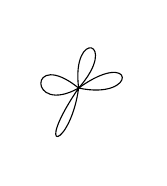
\begin{tikzpicture}[scale=0.8]
\draw (0,0) .. controls (-0.8,0.65) and (-0.8,-0.45) .. (0,0);
\draw (0,0) .. controls (-0.12,0.95) and (0.66,0.75) .. (0,0);
\draw (0,0) .. controls (0.9,0.65) and (0.95,-0.2) .. (0,0);
\draw (0,0) .. controls (-0.13,-0.95) and (-0.75,-1.1) .. (0,0);
\end{tikzpicture}
\end{adjustbox}
\end{center}

[Слева зачёркнуто:
\Incomplete{GELFAND-P000475}{lower-left-cancelled}{Короткая запись перед строкой с $H^{n-1}$ не прочитана под плотной штриховкой.}]
$H^{n-1}$ имеет образующие $e_1\ e_2\ldots\ e_\mu$.

Индекс пересеч. опред. скалярное произвед. $(e_i,e_k)$.

$n-1\equiv2\pmod4$\qquad\underline{$e_i^2=-2$} (всегда)

[За двойной вертикальной чертой, в столбик:]

отриц. опред.

полуопред.

[Зачёркнутая строка:
\Incomplete{GELFAND-P000475}{lower-signature-cancelled}{Запись непосредственно под «полуопред.» не прочитана из-за густого зачёркивания.}]

неопред.

\underline{Монодромия}: предст. фунд. гр. в
[зачёркнуто:
\Incomplete{GELFAND-P000475}{lower-monodromy-cancelled}{Слово после «в» почти полностью перекрыто чертами.}]
\ldots

[Разделитель: две толстые черты с точкой между ними.]

[Зачёркнуто: \Unclear{GELFAND-P000475}{bottom-cancelled-name}{Атья}.]

\underline{Есть раб. Атья, Ботта,\ldots:} как избавиться от производных
в выкладках Синг. Как, сидя в одной точке, изучить топологию
мира? Нахожд. явного вида асимптотики для ур-й 2-го
порядка (сообр. И. М. Гельфанда, В. И. Арнольда и др.)

(будет в следующем семестре)

А. Шнирельман о работах Маслова.

\SourcePage{GELFAND-P000476}{unlabelled}
\underline{\underline{В. М. Бухштабер.}} (продолжение).
\begin{gather*}
A\overset{\text{аддит.}}{\simeq}\Lambda[[X]],
\qquad X_n\text{ --- аддит. образующие}\\
X_n\cdot X_m=C_{n+m}^{n}X_{n+m}
\end{gather*}
\begin{equation*}
\operatorname{Ext}_A^{2,*}(\Lambda,\Lambda)
=\ker d_3^*/\operatorname{Im}d_2^*
\qquad\text{в терминах $B$-конструкции}
\end{equation*}
$1^{\circ}$.\quad
$d_3^*:\bar A^*\otimes\bar A^*\longrightarrow
\bar A^*\otimes\bar A^*\otimes\bar A^*$

\Unclear{GELFAND-P000476}{top-dual-hom}{$A^*=\operatorname{Hom}_{\Lambda}^{c}(\Lambda[[X]],\Lambda)
\overset{\text{адд.}}{\simeq}\Lambda[x]$}

[Под обозначением $\operatorname{Hom}$ приписано:]
\underline{\underline{компактное}} (ненулев. знач. на конечн. числе).
\begin{equation*}
\Delta:A^*\longrightarrow A^*\otimes A^*
\end{equation*}
\Unclear{GELFAND-P000476}{top-delta-star}{$\displaystyle
\Delta x_n\longrightarrow x_n\otimes1+1\otimes x_n+
\sum d_{i,j}\,x_i\otimes x_j^*$}
\begin{gather*}
(\Delta x_n,x_i\otimes x_j)=d_{i,j}\\
(x_n,x_i\cdot x_j)=(x_n,C_{i+j}^{i}x_{i+j})=C_{i+j}^{i}\delta_{n,i+j}
\end{gather*}
[Между первыми скобками двух строк поставлен вертикальный знак равенства.]
\begin{equation*}
\Delta x_n=x_n\otimes1+1\otimes x_n+
\sum C_n^i x_i\otimes x_{n-i}
\end{equation*}
И положим\quad $x_n=x^n$
\begin{gather*}
\Delta x^n=(x\otimes1+1\otimes x)^n\\
d_3^*:\overline{\Lambda[x,y]}\longrightarrow\overline{\Lambda[x,y,z]}
\end{gather*}
\Unclear{GELFAND-P000476}{middle-differential-star}{$\displaystyle
 d_3(h(x,y))=\sum h_{ij}(\bar\Delta x^i)z^j
 -\sum h_{i,j}x^i\bar\Delta y^j=$}

[Под $h(x,y)$, со знаком равенства:]
$\sum h_{i,j}x^iy^j$
\begin{equation*}
\bar\Delta x^n=\Delta x^n-x^n-y^n.
\end{equation*}
[Под $\Delta x^n$ последовательно, с вертикальными знаками равенства:]
\begin{gather*}
(\Delta(x))^n\\
(x+y)^n
\end{gather*}
[Продолжение строки вычисления:]
\begin{multline*}
=h(x+y,z)\overset{\text{зачёркнуто}}{-h(x,z)}-h(y,z)
-h(x,y+z)+h(x,y)\overset{\text{зачёркнуто}}{+h(x,z)}.
\end{multline*}

\underline{\underline{$\ker d_3^*$:}}\quad
\fbox{$h(x+y,z)+h(x,y)=h(x,y+z)+h(y,z)$}
\quad эти циклы обозн. $L$.

Это и есть Лазаровское соотношение.
\begin{gather*}
\underline{\operatorname{Im}d_2^*}=\Lambda\{d_2^*x^n\}\\
0\longrightarrow\operatorname{Im}d_2^*\longrightarrow L
\longrightarrow\operatorname{Ext}_A^{2,n}(\Lambda,\Lambda)\longrightarrow0
\end{gather*}
\underline{Счёт группы $\operatorname{Ext}$.}

В ур-ии не фигурирует $\Lambda$. Поэтому дост. счит. 2 случая:

1)\quad $\Lambda$ --- $Z_p$-модуль ($p$ --- простое)

2)\quad $\Lambda=Q$

\SourcePage{GELFAND-P000477}{unlabelled}
остаётся\quad $X_{p^i}$

\Unclear{GELFAND-P000477}{top-tensor-product}{\underline{$A=\widehat{\prod}\otimes A_i$}},
\qquad $A_i=Z_p[X_{p^i}]/(X_{p^i}^{p})\otimes_{Z_p}\Lambda$
\begin{gather*}
H^*(A_i)=\Lambda_p(u_i)\otimes Z_p[v_i],\quad
\operatorname{deg}u_i=p^i,\quad\operatorname{deg}v_i=p^{i+1}\\
u_i\in\operatorname{Ext}^{1,p^i};\qquad
v_i\in\operatorname{Ext}^{2,p^{i+1}}
\end{gather*}
\Unclear{GELFAND-P000477}{top-generator-inequality}{$\operatorname{Ext}_A^{2,*}
=\{u_i u_j,\ i<j,\ v_k\}$.}

[Под перечнем скобкой объединена подпись:]
\underline{образующие}

[Зачёркнуто: \Unclear{GELFAND-P000477}{middle-cancelled-word}{Это}.]
Но: нужны симметрич.\quad\underline{$h(x,y)=h(y,x)$}

\underline{\underline{Бывают некоммут. одномерные группы!!}}
(если есть кручение)

(соотв. циклам $u_i u_j$)

\underline{Пример:}\quad $x+y+axy^p$, где $a^2=0$
\quad над $Z_p[a]/(a^2)$.

Это некоммут. форм. группа!!

Их столько, сколько циклов.

$v_k$ соотв. коммут. группы
\begin{equation*}
h(x,y)=(x+y)^{p^{k+1}}-x^{p^{k+1}}-y^{p^{k+1}}
\end{equation*}
коэфф. дел. на $p$ (\Unclear{GELFAND-P000477}{bottom-divisibility-word}{только})
\begin{equation*}
\underline{L_{p^{k+1}}(x,y)=\frac{h(x,y)}{p}}
\end{equation*}
\underline{(в $\forall$ размерности по 1-й образующей)}

\underline{В этом семестре конец.}

\SourcePage{GELFAND-P000478}{unlabelled}
\underline{12/II-73г.}\qquad\underline{Сем. Гельфанда.}

\underline{План:}\quad 1. Бухштабер; Мищенко: Топология (раб. Сулливана)

2. Раб. Делиня, Ленглендса

\underline{В. Бухштабер.}\qquad\underline{О 1-й раб. Сулливана.}

$M^n$ --- мн-зие

Гладкость $M^n$ --- это гл. мн-зие $N^n$ и гомот. эквив.
$N^n\overset{f}{\longrightarrow}M^n$
\begin{center}
\begin{adjustbox}{max width=\linewidth}
\begin{tikzcd}
N_1^n \arrow[r,"f_1"] \arrow[d,"g"'] & M^n \\
N_2^n \arrow[ur,"f_2"'] &
\end{tikzcd}
\end{adjustbox}
\end{center}
Эквивал. $\Longleftrightarrow\exists$ диффеом. $g$, такой, что этот
квадрат коммутативен (гомотопически).

$S(M^n)$ --- мн-во классов эквив. гладкостей.

[Над именем зачёркнуто:
\Incomplete{GELFAND-P000478}{top-milnor-cancelled}{Короткая запись над «Милнор» не прочитана из-за плотной штриховки.}]

\underline{Милнор:}\quad $\operatorname{Card}S(S^7)=28$.

Описание\quad $S(M^n)$ --- ?

\underline{Сулливан} рассм. в $M^n$ фиксир. кусочно-линейную структуру.

[Справа под строкой:]
($M^n$ --- полиэдр)

\underline{и решил зд. в этой постановке:}

(вместо диффеом. --- кусочно-лин.
[зачёркнуто: \Incomplete{GELFAND-P000478}{middle-cancelled-homeo}{Короткий фрагмент перед «гомеоморфизм» не прочитан.}]
гомеоморфизм)

Получ.\quad $PL(M^n)$.

Здесь всегда\quad\underline{\underline{$PL(S^n)=\{S^n\}$}}
--- там, где решена пробл. Пуанкаре (при $n\ge5$).

Рассм. на $M^n$
[зачёркнуто: \Incomplete{GELFAND-P000478}{middle-vector-cancelled}{Запись перед словом «расслоение» закрашена;} сверху вписано и обведено: вект.]
расслоение $\xi$, стабильное (большой разм.).

[Зачёркнуто:
\Incomplete{GELFAND-P000478}{middle-cancelled-phrase}{Первое слово предположительно «несколько»; среднее слово не прочитано.}
тривиальное]

$T_\xi$ --- комплекс Тома рассл. $\xi$,
\qquad\fbox{$T_\xi=\dfrac{D(\xi)}{S(\xi)}$}

[Справа:] $D$ --- рассл. шаров,

$S$ --- рассл. сфер.

$\dim\xi=m$.
\begin{equation*}
S^m\overset{i}{\subset}T_\xi
\end{equation*}
[Подпись снизу:] \underline{в точке.}
\begin{center}
\begin{adjustbox}{max width=\linewidth}
\begin{tikzcd}
\mathbb R^m \arrow[r] \arrow[d] & \xi \arrow[d] \\
* \arrow[r,hook] & M^n
\end{tikzcd}
\end{adjustbox}
\end{center}

Рассл. $\xi$ наз. $J$-тривиальным, если $\exists$ отобр. $\varphi$,
такое что

\SourceFigure{GELFAND-P000478}{lower-j-diagram}{Слева направо видны $S^m$, стрелка к $T_\xi$ с исправленной подписью $i$, затем стрелка с подписью $\varphi$ к $S^m$. У последней сферы снизу справа густо обведённый знак, похожий на отменённый индекс или звёздочку. Снизу от левой сферы идёт дугообразная стрелка к правой, под дугой написано $1$. Справа и под второй стрелкой большой зачёркнутый участок с остатками прежних линий и букв; его содержимое и прежнюю геометрию восстановить уверенно нельзя.}

(гомот.)

т. е.\quad $\operatorname{deg}(\varphi i)=1$

(от выбора $*$ ничего не зависит, т. к. $M^n$ предполаг. связным).

$K_J(M^n)$ --- группа стаб. рассл. над $M^n$, каждое из
к-рых $J$-тривиально
\SourcePage{GELFAND-P000479}{unlabelled}
\underline{Теор. Атьи:} (Мат. 10:5)

стр. отобр.
[Зачёркнуто: \Unclear{GELFAND-P000479}{top-erasure}{выражение, начинающееся с $S$; остальное неразборчиво}.]
\begin{equation*}
\underline{S(M^n)\longrightarrow K_J(M^n).}
\end{equation*}
\begin{equation*}
N^n\longrightarrow M^n \qquad \underline{\text{разность.}}
\end{equation*}

[Зачёркнуто: Сулливан:
\begin{equation*}
0\longrightarrow PL(M^n)\longrightarrow K_{PLJ}(M^n)
\end{equation*}
всегда.]

и
\begin{equation*}
0\longrightarrow PL(M^n)\longrightarrow K_{PLJ}(M^n)
\end{equation*}
[В конце строки зачёркнуто: \Unclear{GELFAND-P000479}{line-erasure}{$\to0$?}.]
\begin{equation*}
\text{при}\quad n\equiv\hspace{-0.75em}/\;0,2\bmod4
\end{equation*}
\begin{equation*}
\begin{array}{lll}
n\equiv0\bmod4 & \text{коядро} & Z\\
n\equiv2\quad\text{—//—} & \text{—//—} & Z_2.
\end{array}
\end{equation*}
Сулливан выч. гомот. \Unclear{GELFAND-P000479}{group-word}{груп / групп}
предст. пр-ва $K_{PLJ}(M^n)$.

Для $K_J(M^n)$ не сделано. Послед. для $S(M^n)$ тоже есть.

\SourcePage{GELFAND-P000480}{unlabelled}
\underline{19/II-73.}\qquad \underline{Р. Л. Добрушин.}

\underline{О теории поля.}

\underline{Гельфанд:} 2 задачи:

1) проквантовать \Unclear{GELFAND-P000480}{tasks-existing}{существующ. / существ.} ур-я

2) напис. ур-я, реально \Unclear{GELFAND-P000480}{tasks-answering}{отвеч. / ответ.} (физ.)

\underline{Способ констр. объектов, удовл. аксиомам Уайтмана}
(\underline{вероятн. объекты}).

Осн. автор --- \underline{Nelson}.

Можно (почти) получ. рез. Глимма и Джаффе.

Случ. величина: $\xi_t$,\quad
\Unclear{GELFAND-P000480}{field-index}{$t\in R^{\nu+1}$ / $t\in R^{v+1}$}.

1) она евкл. инвар.

2) Марк. св-во

\SourcePage{GELFAND-P000481}{unlabelled}
\underline{26/II-73}\qquad \underline{В. М. Бухштабер.}

$hs(M^n)$ --- [вставлено над словом: гомотопич.] гладкости.

\underline{$ht(M^n)$} --- гомот. триангуляции.

[Под $ht(M^n)$, соединено чертой: \underline{описывается.}]

\underline{Hauptvermutung} --- гомеоморфизм [вставлено: мн-зий]
можно заменить кусочно-лин. гомеом.
(если $M$ односв. и не имеет в $H^3$ 2-кручения)

Пусть $\alpha\in hs(M^n)$ (гом. гладкость).
\begin{equation*}
\alpha\mapsto\underbrace{\xi\longrightarrow M^n}_{\text{расслоение (вект.)}}
\qquad\underline{\text{гладкое.}}
\end{equation*}
[Под первой стрелкой: \Unclear{GELFAND-P000481}{assigned}{сопост. / сопст.}]
\begin{equation*}
f\colon N^n\longrightarrow M^n;
\end{equation*}
\begin{equation*}
\exists\ g\colon M^n\longrightarrow N^n;\qquad
f\circ g\sim1,\quad g\circ f\sim1.
\end{equation*}
\begin{equation*}
\tau_{M^n}+g^*\nu_{N^n}
\qquad(\nu_{N^n}=-\tau_{N^n}\bmod\text{трив.})
\end{equation*}
\underline{Упр.} Док., что 2 экв. гладкости индуц. изом. расслоения $\xi$.

Получ. гладкое рассл. $\xi$ явл. $J$-тривиальным, т.е.
\begin{equation*}
\begin{adjustbox}{max width=\linewidth}
\begin{tikzcd}
\xi \arrow[r,"\gamma"] \arrow[d] & M^n\times R^N \arrow[d] \\
M \arrow[r,"\mathrm{id}"'] & M
\end{tikzcd}
\end{adjustbox}
\end{equation*}
и $\gamma$ есть собственное отбр. и гомот. эквивал.

[Зачёркнуто: $T(\xi)$ \Unclear{GELFAND-P000481}{cancelled-word}{эквив. / трив.}.]

\underline{2-е опр.} --- $\exists$ отобр. $T(\xi)\longrightarrow S^N$,
такое что

[Над $T(\xi)$, со стрелкой к нему: \underline{комп. Тома}.]

композиция
\begin{equation*}
\begin{adjustbox}{max width=\linewidth}
\begin{tikzcd}[column sep=large]
S^N \arrow[r,phantom,"\subset"] \arrow[rr,bend right=20] &
T(\xi) \arrow[r] & S^N
\end{tikzcd}
\end{adjustbox}
\end{equation*}
есть гомотопич. эквив.

Эквивалентность --- теор. \underline{\Unclear{GELFAND-P000481}{dold-name}{Долда / Дольда}}
(технич., идейно трив.)

\SourcePage{GELFAND-P000482}{unlabelled}
\underline{5/III-73 г.}\qquad \underline{Сем. Гельфанда.}

\underline{Теорема.}
[Зачёркнуто: \Unclear{GELFAND-P000482}{cancelled-name}{Ф. А. Березин?}.]
\underline{Ломоносов.}

$R$ --- сем-во попарно комм. опер.
[вставлено: в бан. пр-ве $B$], содержащее вп. непр. опер.
\Unclear{GELFAND-P000482}{operator-condition}{$A\ne C$ / $A\ne0$}.
Тогда $R$ имеет общее [вставлено: нетрив.] инвариантное подпр-во.

(обобщение теоремы \Unclear{GELFAND-P000482}{theorem-name}{Ароншайна / Аронштайна} --- Смита)

Док-во проходит в случае ЛВП, и короткое и простое.

\underline{Док-во.}
\Unclear{GELFAND-P000482}{ball-prime}{$S'$ / $S$} --- замкн. шар
[вставлено: в $B$], $r=1$ с центром в $x_0$, такой, что
\begin{equation*}
\inf_{x\in S}\lVert Ax\rVert>1/2
\end{equation*}
\begin{equation*}
\begin{gathered}
Ax_0'\ne0\\
\lVert x_0'\rVert=1
\end{gathered}
\end{equation*}
и берём
\Unclear{GELFAND-P000482}{scaling}{$\lVert A\rVert\cdot x_0'=x_0$.}

$\overline{AS}$ --- компакт, не содержащий нуля.

Рассм. алгебру [вставлено: $\mathcal R$] с $1$,
порожденную сем-вом $R$ (без замыкания).
\begin{equation*}
\forall y\in B,\qquad \mathcal R y\quad\text{--- лин. мн-зие.}
\end{equation*}
Легко видеть, что $\mathcal R y$ инвар. отн. $\mathcal R$.

$\overline{\mathcal R y}$ --- инв. подпр-во.

Надо док., что оно может быть нетрив.

Пусть $y\in\overline{AS}$. Надо пров., что $\exists y$;
$\mathcal R y$ не плотно.

Пусть не так, тогда
[зачёркнуто: \Unclear{GELFAND-P000482}{then-erasure}{оно?}]
\begin{equation*}
\forall y\in\overline{AS}\quad\exists T\in\mathcal R,
\qquad\lVert Ty-x_0\rVert<1.
\end{equation*}
Из комп. $\overline{AS}$ след. $\exists T_1,\ldots,T_n$
\begin{equation*}
\forall y\ \exists i\qquad\lVert T_i y-x_0\rVert<1,
\end{equation*}
\begin{equation*}
\forall y\in AS\quad\{T_1y,\ldots,T_ny\}\cap S\ne\varnothing.
\end{equation*}
Пусть $f(t)\in C(0,+\infty)$

% Source drawing: original pixels (1040,3060)-(1610,3300); checked at 3x.
\begin{center}
\begin{adjustbox}{max width=\linewidth}
\begin{tikzpicture}[x=1.1cm,y=1.1cm]
\draw[->] (-0.2,0)--(3.6,0) node[right] {$t$};
\draw (0,0)--(0,1.25);
\draw[thick] (0,1)--(1,0);
\fill (1,0) circle (1.1pt);
\node[left] at (0,1) {$1$};
\node[below] at (1,0) {$1$};
\node[right] at (0.4,1.1) {$f(t)$};
\end{tikzpicture}
\end{adjustbox}
\end{center}

\SourcePage{GELFAND-P000483}{unlabelled}
Рассм.
\begin{equation*}
\Phi y=\frac{\displaystyle\sum_1^n f(\lVert T_i y-x_0\rVert)T_i y}
{\displaystyle\sum_j f(\lVert T_j y-x_0\rVert)}
\qquad(\text{вып. комб.})
\end{equation*}
[Перед верхней чертой знака равенства:
\Unclear{GELFAND-P000483}{definition-mark}{плотный значок, похожий на $\#$ или $*$}.]
\begin{equation*}
\Phi\colon\overline{AS}\longrightarrow S
\end{equation*}
Это непр. ф-я на $\overline{AS}$.

Рассм. $\Phi A$
[затёрт знак: \Unclear{GELFAND-P000483}{after-phi-a}{$x$?}]
$\colon S\longrightarrow S$,

причём образ $\Phi A$ компактен и оно непр.

По теор. Шаудера $\exists$ неподв. точка, т.е.
\begin{equation*}
\sum_1^n\alpha_i T_i Ax=x,\qquad
\alpha_j=\frac{f(\lVert T_jy-x_0\rVert}
{\displaystyle\sum_i f(\lVert T_i y-x_0\rVert)}
\end{equation*}
\Unclear{GELFAND-P000483}{weights}{В формуле для $\alpha_j$: $x_0$ / $x$;
в числителе закрывающая скобка после нормы не видна.}

\underline{$T=\sum\alpha_i T_i A$ вп. непрерывен.}

$\exists x\colon Tx=x$. Отсюда соб. вект. с соб. знач. $1$ ---
нетрив. инвар. подпр-во (даже конечномерное).
Отсюда $\mathcal R$ имеет инвар. подпр-во.
[Росчерк: небольшой овал над двумя перекрещивающимися штрихами, справа точка.]

(Это не значит, что вообще есть конечномерное).

\underline{Следствие.}
Если комм. [вставлено: бан.] алгебра имеет элем.,
[затёртые знак и слово:
\Unclear{GELFAND-P000483}{corollary-cancel}{первый знак похож на и; слово неразборчиво}]
умн. [вставлено: на к-рый] вп. непр.,
то $\exists$ нетрив. идеал.

\medskip
\underline{Хенкин.}\ (\underline{анонс})

Пусть в $C^n$ есть вып. обл. $D\subset C^n$, зад. ур-ем $\rho(z)<0$.

Интегр. ф-ла Лерэ для голом. огран. ф-й:
\begin{equation*}
f(z)=\frac{(n-1)!}{(2\pi i)^n}
\int_{\zeta\in\partial D}
\frac{f(\zeta)\,\omega'\bigl(\frac{\partial\rho}{\partial z}(\zeta)\bigr)
\wedge\omega(\zeta)}
{\bigl(\displaystyle\sum_{k=1}^n
\frac{\partial\rho}{\partial\zeta_k}(\zeta)(\zeta_k-z_k)\bigr)^n}
\end{equation*}

1) Инт. типа Лерэ:
\begin{equation*}
f_g(z)=\cdot\ \cdot\ \int
\begin{matrix}g(\zeta)\cdots\\ \cdots\end{matrix}
\qquad g(\zeta)\text{ --- ф-я на границе.}
\end{equation*}
\begin{equation*}
f\longrightarrow[f(\zeta)g(\zeta)-f_g(\zeta)]
\quad\text{--- вп. непр. оператор}
\end{equation*}
и усл. Гёльдера с показ. $1/2$

2) $\rho(z)$ --- строго плюрисубгарм.

% Left contour: original pixels (250,2580)-(400,2740); checked at 3x.
\begin{adjustbox}{max width=\linewidth}
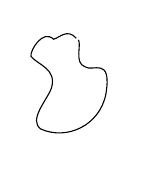
\begin{tikzpicture}[x=0.7cm,y=0.7cm]
\draw (0.18,1.2)
.. controls (0.02,1.38) and (-0.12,1.21) .. (-0.23,1.18)
.. controls (-0.42,1.37) and (-0.66,0.98) .. (-0.64,0.87)
.. controls (-0.53,0.72) and (-0.16,0.65) .. (-0.27,0.29)
.. controls (-0.36,0.06) and (-0.69,-0.29) .. (-0.46,-0.45)
.. controls (0.02,-0.66) and (0.61,-0.38) .. (0.72,0.19)
.. controls (0.83,0.88) and (0.48,0.58) .. (0.34,0.68)
.. controls (0.14,0.75) and (0.28,1.08) .. (0.22,1.17);
\end{tikzpicture}
\end{adjustbox}

Тогда $D$ --- [зачёркнуто: \Unclear{GELFAND-P000483}{domain-cancel}{обл. / область}]
есть замкн. подмн-зие в строго вып. обл.,
трансверс. подх. к границе.

(следует из теор. Ока)

\SourceFigure{GELFAND-P000483}{domain-right}{Справа нарисован наклонный овал
с внутренней дугой. Дуга подходит к верхнему краю и оканчивается
вблизи нижнего; нужно проверить, обозначает ли рисунок касание
границы в обоих концах. Подписей и стрелок не видно.}

3) в п. 2) \underline{выпис. продолж. с подмн-зия с оценками!}
(в классе огр. ф-й)

Обратное тоже верно: такое подмн-зие есть
[зачёркнуто: \Unclear{GELFAND-P000483}{converse-cancel}{обл. / область}]
огр. область голоморфности.

4) \underline{Следствие:} для ф-й, ан. внутри и непр. в замыкании,
пр-во макс. идеалов $=$ замыканию области.

\SourcePage{GELFAND-P000484}{unlabelled}
\underline{Ф. А. Березин.}

\underline{Зад. квантования.}

$M$ --- симпл. мн-зие
($\omega$ --- форма \Unclear{GELFAND-P000484}{form-mark}{$2$ / $\xi$ / затёртый знак}
с матр. $\omega_{ik}$; $\omega^{ik}$ --- обр. матр.)
\begin{equation*}
[f,g]=\sum\omega^{ik}\frac{\partial f}{\partial x^i}
\frac{\partial g}{\partial x^k}
\end{equation*}
Квантование: сем-во ассоц. колец $A_h$ с элементами $f(x)$ (ф-и на $M$)
\begin{equation*}
f_1\ast f_2=g(x\mid h)
\end{equation*}
\begin{equation*}
\left.
\begin{aligned}
1)\quad &g(x\mid0)=f_1(x)\cdot f_2(x)\\
2)\quad &\left.\frac{\partial}{\partial h}
(f_1\ast f_2-f_2\ast f_1)\right|_{h=0}=[f_1,f_2]
\end{aligned}
\right\}\quad(\text{принцип соответствия}).
\end{equation*}
Ещё ряд треб. (не столь обяз.)

3) все $A_h$ --- алгебры с $1$, соотв. $f_0\equiv1$.

4) $A_h$ --- алгебра со следом (опр. на выд. мн-ве элементов
[окончание переписано: \Unclear{GELFAND-P000484}{trace-domain}{прежнее чтение неразборчиво}]
в $A_h$).
\begin{equation*}
\mathrm{Sp}(f_1\ast f_2)=\mathrm{Sp}(f_2\ast f_1)
\end{equation*}
и
\begin{equation*}
\mathrm{Sp}\,f=c\int f\,d\mu,
\end{equation*}
где $d\mu$ --- ест. мера на мн-зии
(\Unclear{GELFAND-P000484}{measure-word}{определена / определено} $\omega$).

Треб. мат. естеств. --- \underline{функториальность} по отн. к каноническим
Диффеоморфизмам (отн. нек-рого сем-ва отобр. --- нек-рой фикс. категории).

\medskip
Решение изв., когда $M\in$ опр. классу
(2 класса кэлеровых мн-зий).

[Объединены скобкой:]

1) обл. в $C^n$

2) компактные симм. мн-зия,

[Над началом следующего заголовка — закрашенная отметка.]

\underline{Фоковское пр-во.}
\begin{equation*}
M=C^n\qquad\omega=\sum dz_i\wedge d\bar z_i.
\end{equation*}
Ф-и --- целые ф-и $f(z,\bar z)$
(разл. по $x,y$ в ряд, всюду сход.)
\begin{equation*}
(f_1\ast f_2)(z,\bar z)=\frac1{h^n}
\int f_1(z,\bar v)f_2(v,\bar z)
 e^{-\frac1h(z-v)(\bar z-\bar v)}\,dv\,d\bar v
\end{equation*}
Важно: строение лин. предст. этого кольца.

Пусть $\varphi(z)$ --- обычные целые ф-и с усл.
\begin{equation*}
(\varphi,\varphi)=\frac1{h^n}
\int|\varphi(z)|^2e^{-\frac{z\bar z}{h}}\,dz\,d\bar z
<+\infty\qquad(\text{пр-во }F_2)
\end{equation*}
Там действует лин. предст. кольца $A_h$:
\begin{equation*}
(\hat f\varphi)(z)=\frac1{h^n}\int
 f(z,v)\overline{\varphi(v)}\,
 e^{-\frac1h(v-z)\bar v}\,dv\,d\bar v,
\end{equation*}
$f$ --- виковский символ.

\Unclear{GELFAND-P000484}{wick-conjugation}{В рукописи: $f(z,v)$ без черты над $v$,
и черта над $\varphi(v)$.}

Ещё одно кольцо операторов:
\begin{equation*}
(\hat f\varphi)(z)=\frac1{h^n}\int
 \mathring{f}(v,\bar v)\varphi(v)
 e^{-\frac1h(v-z)\bar v}\,dv\,d\bar v,
\end{equation*}
$\mathring{f}$ --- антивиковский символ.
\begin{equation*}
(\hat a_k\varphi)(z)=\frac{\partial\varphi}{\partial z_k},
\qquad(\hat a_k^*\varphi)(z)=z_k\varphi.
\end{equation*}
[Надстрочный знак при первом $\hat f$:
\Unclear{GELFAND-P000484}{ordered-erasure}{$*$ / затёртый знак}.]
\begin{equation*}
\hat f=\sum f_{mn}\hat a^{*m}\hat a^n
\longleftrightarrow
f(z,\bar z)=\sum f_{mn}\bar z^m z^n
\end{equation*}
\begin{equation*}
\hat f=\sum\mathring{f}_{mn}\hat a^n\hat a^{*m}
\longleftrightarrow
\mathring{f}(z,\bar z)=\sum\mathring{f}_{mn}z^n\bar z^m.
\end{equation*}
\Unclear{GELFAND-P000484}{ordering-bars}{Порядок степеней и черты над $z$
оставлены как в рукописи; показатель $n$ в нижней строке местами затёрт.}

\SourcePage{GELFAND-P000485}{unlabelled}
Рассм. $e_{\bar v}(z)=e^{\frac{1}{h}\bar v z}$
(когерентные сост. или пуасс. векторы).

[Зачёркнуто: \Unclear{GELFAND-P000485}{upper-erasure}{$f\ldots$; остальное неразборчиво.}]
Рассм. теперь
\begin{equation*}
\begin{aligned}
\hat f&\longleftrightarrow f(v,\bar v)
 =\frac{(\hat f e_{\bar v},e_v)}{(e_{\bar v},e_v)}
 \quad\text{(распространение)}={}\\
 &\hspace{11em}{}=\operatorname{Sp}(\hat f P_v).
\end{aligned}
\end{equation*}
\Unclear{GELFAND-P000485}{coherent-subscripts}{В числителе и знаменателе у первого $e$ написано $\bar v$, у второго --- $v$ без черты.}

($P_v$ --- ортог. проект. на $e_v$)
\begin{equation*}
\hat f=\int\mathring f(v,\bar v)P_v\,dv\,d\bar v
\qquad\text{(распр. антивик. символов).}
\end{equation*}

\underline{Двойственность:}

1.
\begin{equation*}
\begin{array}{lll}
\text{вик.}&\text{оп.}\longrightarrow\text{символ}\\
\text{антивик.}&\text{симв.}\longrightarrow\text{оператор}
\end{array}
\end{equation*}
\SourceFigure{GELFAND-P000485}{duality-vertical-mark}{Перед «оп.» виден густо обведённый вертикальный знак со стрелкой вверх; верхушка подходит к подчёркиванию заголовка «Двойственность». Связь этого знака с двумя строками не установлена.}

2.
\begin{equation*}
\begin{aligned}
\hat f\text{ --- огр.}&\Longrightarrow f\text{ огр.}\\
\mathring f\text{ --- огр.}&\Longrightarrow\hat f\text{ огр.}
\end{aligned}
\end{equation*}

3.
\begin{equation*}
\begin{aligned}
\hat f\text{ комп.}&\Longrightarrow f\to0\\
\mathring f\to0&\Longrightarrow\hat f\text{ комп.}
\end{aligned}
\end{equation*}

4. Ядерность (анал.)
\begin{equation*}
\operatorname{Sp}\hat f
 =\frac{1}{h^n}\int f(z,\bar z)\,dz\,d\bar z
 =\frac{1}{h^n}\int\mathring f(z,\bar z)\,dz\,d\bar z.
\end{equation*}

\underline{Ф-ла перехода:}
\begin{equation*}
f(z,\bar z)=\frac{1}{h^n}\int\mathring f(v,\bar v)
 e^{-\frac1h(z-v)(\bar z-\bar v)}\,dv\,d\bar v.
\end{equation*}
При $h/2$ получается символ Вейля.
(Замеч. Гельфанда: [вписано сверху, со знаком вставки: это символы] Пуанкаре.)

\underline{\underline{Общая конструкция.}}

$H$ --- гильб. пр-во, $M$ --- мн-во с мерой, $\alpha\in M$, мера $d\alpha$.

$e_\alpha$ --- переполн. сист., если
\begin{equation*}
(f,f)=\int |(f,e_\alpha)|^2\,d\alpha.
\end{equation*}
Рассм. тогда соответствие:
\begin{equation*}
\hat A\longrightarrow\frac{(\hat A e_\alpha,e_\alpha)}{(e_\alpha,e_\alpha)}
 =A(\alpha)\qquad\text{(ковар. символ)}.
\end{equation*}
[Под $A(\alpha)$ повторительные штрихи и запись:]
\begin{equation*}
\operatorname{Sp}(\hat A\hat P_\alpha).
\end{equation*}
контравар. символ.
\begin{equation*}
\hat A=\int\mathring A(\alpha)\hat P_\alpha\,d\alpha.
\end{equation*}
Раньше: $e_\alpha=e^{\bar v z}$, $\alpha=(v,\bar v)$.

Все теор. справедливы.

\underline{Другой способ:}

$H\hookrightarrow L^2(M)$, $\hat T$ --- ортог. проектор $L^2(M)$ в $H$.
\Unclear{GELFAND-P000485}{embedding-overwrite}{Знак между $H$ и $L^2(M)$ густо обведён; читается как стрелка включения вправо.}
\begin{equation*}
(\hat Bf)(\alpha)=\mathring A(\alpha)f(\alpha)
\quad\text{--- оператор в }L^2(M).
\end{equation*}
Тогда
\begin{equation*}
\underline{\hat A=\hat T\hat B\hat T.}
\end{equation*}

\SourcePage{GELFAND-P000486}{unlabelled}
\underline{\underline{Пример:}} $e^{i(p,x)}$ в огр. областях.

Пусть $\varphi(x)$ --- произв. вып. [вписано сверху: вниз] ф-я вещ. перем. $x$.
[Под «вып.» нарисована дуга, выпуклая вниз.]

Тогда
\begin{equation*}
\underline{\int\varphi(A)\,d\mu\leq\operatorname{Sp}\varphi(\hat A)
 \leq\int\varphi(\mathring A)\,d\alpha}.
\end{equation*}
\Unclear{GELFAND-P000486}{left-differential}{В левом интеграле дифференциал читается $d\mu$ или $d\alpha$.}

Лев. часть --- следствие нер-ва Йенсена.

Прав. часть --- \Unclear{GELFAND-P000486}{before-trace}{короткий густой знак: стрелка вправо или зачёркнутый знак.}
\begin{center}
\fbox{$\operatorname{Sp}(P\varphi(A)P)\geq\operatorname{Sp}\varphi(PAP)$}
\end{center}
\Unclear{GELFAND-P000486}{trace-parenthesis}{В правой части скобка после $\varphi$ слита с соседними штрихами; чтение $\operatorname{Sp}\varphi(PAP)$.}

Рассм. область $\underline{G\subset\mathbb C^n}$,

в ней сущ. естеств. [вертикальный штрих] Кэлерова метрика.

Строим кольцо [зачёркнуто: \Unclear{GELFAND-P000486}{ring-erasure}{«от»; либо неразборчивое короткое обозначение.}]
из вещ.-анал. ф-й $f(z,\bar z)$
\begin{equation*}
f_1*f_2=\int f_1(z,\bar v)f_2(v,\bar z)G_h(v,\bar v,z,\bar z)\,dv\,d\bar v,
\end{equation*}
\begin{equation*}
G_h=c(h)\left[\frac{K(z,\bar z)K(v,\bar v)}{K(z,\bar v)K(\bar z,v)}\right]^{1/h},
\end{equation*}
(можно док., что $K(z,\bar v)\ne0$)

где $K$ --- керн-ф-я Бергмана.
\Unclear{GELFAND-P000486}{kernel-quotient}{Дробь записана с диагональными множителями в числителе; во втором множителе знаменателя порядок аргументов $K(\bar z,v)$, показатель $1/h$ без минуса.}

\begin{equation*}
c(h)=h^{-\dim G}c_1(h),
\end{equation*}
$c_1(h)$ непр. при $h\to0$. (любая)

[Стрелка вправо к подчёркнутой помете на поле:]
\underline{неизв. $\exists$ ли квант., удовл. ещё и 3).}

Тогда вып. все треб., кроме 3).

Если $G$ --- однор. обл., то и это тоже вып. и $c_1(h)$ уточняется
[вписано справа в обводках, со знаком вставки: исходя из 3). ест. образом.]

Если $G$ даже симметр., а \underline{дв-ния} --- автом. кольца, то только это.

Переполн. сист. здесь (для однор. обл.)
\begin{equation*}
M=G\subset\mathbb C^n=\mathbb R^{2n}
\end{equation*}
\begin{equation*}
\underline{e_v(z)=(K(z,\bar v))^{1/h}}
\qquad\text{(для однор. области)}.
\end{equation*}
[После степени, ниже неё, зачёркнут знак: \Unclear{GELFAND-P000486}{coherent-exponent-erasure}{неразборчиво; возможно, прежний показатель.}]

Гильбертово пр-во:
\begin{equation*}
H=\{f:\ \int |f(z)|^2K^{1/h}(z,\bar z)\,d\mu(z)<\infty
\quad f\text{ (голом.)}\}.
\end{equation*}
\Unclear{GELFAND-P000486}{hilbert-inequality}{Под знаком $<$ есть густой дополнительный штрих, похожий на зачёркнутое «2»; возможно чтение $\leq$.}
\Unclear{GELFAND-P000486}{hilbert-positive-power}{В весе написано $K^{1/h}$, без видимого минуса перед $1/h$.}

$\mu(z)$ --- инвар. мера, порожд. бергм. метрикой.

Более широкое пр-во --- все ф-и.

В общ. случае неизв., может ли $K(z,\bar v)$ обращаться в $0$.

Ковар. символы: прод-е аналитичны на всё $G\times\bar G$.

\underline{Компактный случай.}
Комп. [вписано сверху, в обводке: комплексное] симметрич. пр-во.

Рассм. потенциал кэлеровой метрики, т.е. $\Phi(z,\bar z)$

\SourcePage{GELFAND-P000487}{unlabelled}
Рассм.
\begin{equation*}
e^{\frac1h\Phi(z,\bar z)}=K_h(z,\bar z)
\qquad
\left(\Phi\text{ опр. усл. }\omega^{ij}=
\frac{\partial^2\Phi}{\partial z_i\partial\bar z_j}\right).
\end{equation*}
При $\underline{h=\frac1n}$ $\Phi(z,\bar z)$ продолж. и сущ. однознач. ф-я
\begin{equation*}
K_h(z,\bar v)
\end{equation*}
и вся предыд. теория.

Тогда гильб. пр-во \Unclear{GELFAND-P000487}{hilbert-symbol}{$H_\alpha$ или $H_h$}
\underline{конечномерно} и $\dim$ легко вычисл.

\underline{Плоск. Лобачевского:}
\begin{equation*}
K^{1/h}=(1-z\bar z)^{+2/h}
\end{equation*}
\Unclear{GELFAND-P000487}{lobachevsky-exponent}{Перед $2/h$ явно написан плюс; знак сохранён.}

Автом. пр-ва порожд. автом. кольца.

Получ. проективное предст. [вписано сверху, в обводке: автом.] плоск. Лобачевского.

\SourcePage{GELFAND-P000488}{unlabelled}
\underline{12/III-73г.}\qquad\underline{Сем. Гельфанда.}

\underline{В.М. Бухштабер.}

$S(M^n)$ --- мн-во гладкостей на $M^n$

$hS(M^n)$ --- гомот. гладкости

$t(M^n)$ --- триангуляции

$ht(M^n)$ --- гом. триангул.

Рассм. мн-во $hS(M^n)$.

На нём рассм. гладкие вект. рассл.
\begin{equation*}
\begin{adjustbox}{max width=\linewidth}
\begin{tikzcd}[row sep=small]
\xi\arrow[d]\\
M^n
\end{tikzcd}
\end{adjustbox}
\end{equation*}
$J$-трив. рассл. (\Unclear{GELFAND-P000488}{fibrewise-word}{посл.; псл.} гомот. трив.), т.е.
\begin{equation*}
\begin{adjustbox}{max width=\linewidth}
\begin{tikzcd}[row sep=small,column sep=large]
\xi\arrow[r,"\varphi"]\arrow[d] & M^n\times\mathbb R^N\arrow[d]\\
M^n\arrow[r,"\mathrm{id}"] & M^n
\end{tikzcd}
\end{adjustbox}
\qquad \underline{\underline{N=\dim\xi}}
\end{equation*}
[Схема подчёркнута снизу, с загнутыми вверх концами линии.]

$\varphi$ --- соб. гомотопич. эквивалентность.

$\Phi(M^n)$ --- мн-во гладких $J$-трив. рассл. на $M^n$
(с точн. до тривиальных).

Пусть
\SourceFigure{GELFAND-P000488}{alpha-map}{Запись $\alpha:\{\ \}$: внутри фигурных скобок слева $N$ с верхним индексом $n$ и густым нижним знаком ($\xi$ или $\zeta$; возможно, исправленный индекс), справа $M^n$. Прямая верхняя стрелка $f$ направлена слева направо; изогнутая нижняя стрелка $g$ --- справа налево. Нижний знак у $N$ не установлен.}
$g$ --- гомот. обр.

По $\alpha$ построим элем. группы $\Phi(M^n)$
\begin{equation*}
\begin{adjustbox}{max width=\linewidth}
\begin{tikzcd}[row sep=large]
\underline{(g^*(\nu_N)+\tau_M)}\arrow[d]\\
M^n
\end{tikzcd}
\end{adjustbox}
\qquad\underline{\underline{\text{оно }J\text{-трив.}}}
\end{equation*}
($\nu_N$ --- норм. пучок $M^n$ --- при влож. в высокомерное пр-во)

инвар. элем. $K$-функтора.
\Unclear{GELFAND-P000488}{normal-bundle-base}{В пояснении к $\nu_N$ написано $M^n$; индекс $N$ и буква $M$ сохранены.}

\begin{equation*}
\begin{aligned}
g\text{ --- тожд.}&\Longrightarrow\nu_N+\tau_M\underset{\mathrm{def}}{=}\text{трив.}\\
g\text{ --- гом. эквив.}&\Longrightarrow\ldots
\end{aligned}
\end{equation*}
[Справа:]
(сложно док. аккуратно ---

--- теор. Атья--Дольда)

Математика 10:5\qquad Пр-ва Тома. (Атья)

Пусть $\pi_1(M^n)=0$.

Точная послед.
\begin{equation*}
hS(M^n)\longrightarrow\Phi(M^n)\longrightarrow P_n
\end{equation*}
\begin{equation*}
P_n=\begin{cases}
0,&n\ne4k,\ 4k+2\\
\mathbb Z,&n=4k\\
\mathbb Z_2,&n=4k+2
\end{cases}
\end{equation*}
\begin{equation*}
\Phi(M^n)\ni\quad
\begin{adjustbox}{max width=\linewidth}
\begin{tikzcd}[row sep=large,column sep=large]
\xi\arrow[r,"\varphi"]\arrow[d] & M^n\times\mathbb R^N\arrow[d]\\
M^n\arrow[r,equal] & M^n
\end{tikzcd}
\end{adjustbox}
\end{equation*}
Добавим $\nu_M$:
\begin{equation*}
\begin{adjustbox}{max width=\linewidth}
\begin{tikzcd}[row sep=large,column sep=large]
\xi+\nu_M\arrow[r,"\varphi\times\mathrm{id}"]\arrow[d] & (M^n\times\mathbb R^N)+\nu_M\arrow[d]\\
M\arrow[r,equal] & M
\end{tikzcd}
\end{adjustbox}
\end{equation*}
$\underline{\varphi\times\mathrm{id}}$ --- соб. гомот. экв.

Отсюда
\begin{equation*}
T(\xi+\nu_M)\longrightarrow T(N+\nu_M)\tag{*}
\end{equation*}
\SourcePage{GELFAND-P000489}{unlabelled}
\underline{Замечание о св-вах комплекса Тома, норм. рассл.}

$M^n\subset R^L$.

\begin{center}
\begin{adjustbox}{max width=\linewidth}
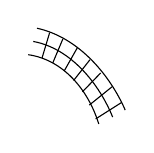
\begin{tikzpicture}[scale=0.8]
\draw (0,0) .. controls (0.55,-0.08) and (0.95,-0.55) .. (1.12,-1.1);
\draw (0.08,0.21) .. controls (0.68,0.1) and (1.13,-0.47) .. (1.34,-0.99);
\draw (0.14,0.42) .. controls (0.82,0.27) and (1.31,-0.35) .. (1.54,-0.88);
\draw (0.22,-0.05) -- (0.34,0.35);
\draw (0.39,-0.13) -- (0.55,0.25);
\draw (0.57,-0.26) -- (0.78,0.11);
\draw (0.72,-0.41) -- (0.98,-0.08);
\draw (0.86,-0.59) -- (1.15,-0.29);
\draw (0.97,-0.80) -- (1.33,-0.51);
\draw (1.07,-1.02) -- (1.48,-0.76);
\end{tikzpicture}
\end{adjustbox}
\end{center}
Пр-во трубки --- пр-во норм. рассл.

Имеется ест. отобр.
\begin{equation*}
\begin{gathered}
\underline{S^L\overset{\lambda}{\longrightarrow}T(\nu_M)},\\
\hphantom{S^L\overset{\lambda}{\longrightarrow}}\cup\\
\hphantom{S^L\overset{\lambda}{\longrightarrow}}M^n
\end{gathered}
\end{equation*}
\Unclear{GELFAND-P000489}{upper-struck-symbol}{[Под левой частью формулы зачёркнут знак: $\beta$ или $\varphi$.]}

Отобр. $\lambda$ трансверс. регулярно на $M^n$. Его прообраз есть $M^n$.
Только это и будет использоваться.

$\exists$ отобр. $S^L\overset{\lambda}{\longrightarrow}T(\nu_M)$
\Unclear{GELFAND-P000489}{upper-cancellation}{[Зачёркнуто: неразборчиво.]}
и вложение $M\subset T(\nu_M)$, к-рое трансверс. регул. на $M$.
\begin{equation*}
\left(
\begin{adjustbox}{max width=\linewidth}
\begin{tikzcd}[column sep=large]
A \arrow[r,"\alpha"] \arrow[rr,bend right=48,swap,"\text{эпи}"] &
\begin{gathered}B\\\cup\\C\end{gathered} \arrow[r] & B/C
\end{tikzcd}
\end{adjustbox}
\right).
\end{equation*}
[Разделитель: короткая черта, точка, короткая черта.]

\underline{Отображение $\varphi(M^n)\longrightarrow P_n$.}
\begin{equation*}
\begin{adjustbox}{max width=\linewidth}
\begin{tikzcd}[column sep=large,row sep=large]
T(N+\nu_M) \arrow[r,dashed,bend left=15,"\sigma"] &
T(\xi+\nu_M) \arrow[l,bend left=15,"\varphi_0"]\\
S^L \arrow[u,"\lambda"] \arrow[ur,"\sigma\circ\lambda"'] &
\end{tikzcd}
\end{adjustbox}
\end{equation*}
\Unclear{GELFAND-P000489}{diagonal-cancellation}{[Под диагональной стрелкой зачёркнуто: предположительно «непр.».]}
$\varphi_0$ по постр. гомот. эквив. $\sigma$ --- гом. обратное.

$\sigma\circ\lambda$ --- непр. отобр. $M\subset T(\xi+\nu_M)$.
Гомотопируем $\sigma\circ\lambda$ [вставлено: в $\widetilde{\sigma\circ\lambda}$],
чтобы оно стало на $M$ трансверс. регул.
\begin{equation*}
\begin{adjustbox}{max width=\linewidth}
\begin{tikzcd}[column sep=large,row sep=small]
S^L \arrow[r,"\widetilde{(\sigma\lambda)}"] & T(\xi+\nu_M)\\
\cup & \cup\\
\underline{M_1=(\widetilde{\sigma\lambda})^{-1}(M)} \arrow[r] & M
\end{tikzcd}
\end{adjustbox}
\end{equation*}
$M_1$ --- гладкое мн-зие. $\dim M_1=\dim M$.

[Зачёркнуто: По теореме Тома $(\widetilde{\sigma\lambda})^{-1}(M)\subset S^L$.]

Важно:
\begin{equation*}
\fbox{$(\widetilde{\sigma\lambda})^*(\xi+\nu_M)=\nu_{M_1}$}.
\end{equation*}
(переформ. трансверс. регулярности)

$\widetilde{\sigma\lambda}:M_1\longrightarrow M$.

Итак, по рассл. $\xi$ мы постр. мн-зие $M_1$ и его непр. отобр.
\begin{equation*}
\begin{gathered}
M_1\longrightarrow M\\
\cap\hphantom{\longrightarrow M}\\
S^L\hphantom{\longrightarrow M}
\end{gathered}
\end{equation*}
$M_1$ с норм. пучком
$\nu_{M_1}=(\widetilde{\sigma\lambda})^*(\xi+\nu_M)$.
(зависит от $\xi$)

\underline{Возникла
\Unclear{GELFAND-P000489}{bottom-cancellation}{[Зачёркнуто: «задача»?]}
ситуация перестройки.}

Задача из гладкой топологии:
насколько однозн. опр. $M_1$.

\SourcePage{GELFAND-P000490}{unlabelled}
\underline{Теор. Милнора --- Кервера.}
Все $M_1$ получ. друг из друга перестр. Морса.

(необх. и дост.)

Сущ. ли там мн-зие, гомот. эквив. $M$.

$P_n$ --- группы препятствий
\Unclear{GELFAND-P000490}{obstruction-cancellation}{[Зачёркнуто: неразборчиво.]}
к перестройкам до гомотопич. эквив.
\begin{equation*}
\underline{\sigma_0:M_1\longrightarrow M}
\end{equation*}
\underline{Послед. точна.}
\begin{equation*}
?\longrightarrow hS(M^n).
\end{equation*}
\begin{equation*}
\begin{aligned}
\alpha_1.&\quad\{N_1\overset{f_1}{\longrightarrow}M\},\\
\alpha_2.&\quad\{N_2\overset{f_2}{\longrightarrow}M\}.
\end{aligned}
\end{equation*}
$\xi_1\in\varphi(M)$ постр. по $\alpha_1$.
\begin{equation*}
\begin{adjustbox}{max width=\linewidth}
\begin{tikzcd}[column sep=large,row sep=large]
\beta_1:S^L \arrow[r] & T(\xi_1+\tau_M) \arrow[d,equal]\\
\beta_2:S^L \arrow[r] & T(\xi_2+\tau_M).
\end{tikzcd}
\end{adjustbox}
\end{equation*}
\Unclear{GELFAND-P000490}{bundle-symbol}{В обозначении $\tau_M$ верхняя волнистая черта может быть частью буквы $\tau$ либо отдельной тильдой: $\tau_M$ или $\widetilde{\tau}_M$.}

Получ. задачи
\Unclear{GELFAND-P000490}{novikov-cancellation}{[Зачёркнуто: неразборчиво.]}
дисс. Новикова:
\begin{equation*}
\begin{gathered}
S^L\times I\longrightarrow T(\xi+\tau_M)\\
\hphantom{S^L\times I\longrightarrow}\cup\\
\hphantom{S^L\times I\longrightarrow}M
\end{gathered}
\end{equation*}
Пленка:
\begin{equation*}
F\big|_{S^L\times0}=\beta_1,\qquad
F\big|_{S^L\times1}=\beta_2.
\end{equation*}
\Unclear{GELFAND-P000490}{last-line-cancellation}{[В начале строки зачёркнут неразборчивый знак.]}
$\exists$ ли среди пленок $h$-кобордизмы?

\SourcePage{GELFAND-P000491}{unlabelled}
% Верхняя большая часть кадра свободна от рукописного текста.
\Unclear{GELFAND-P000491}{date-cancellation}{[Перед датой зачёркнута короткая запись: возможно, цифры.]}
\underline{19/III-73г.}\qquad\underline{Сем Гельфанда}

\SourceFigure{GELFAND-P000491}{annotation-icon}{Над строкой с ростком функции виден жёлтый значок выноски с тремя чёрными горизонтальными штрихами. Текст выноски в данном кадре не раскрыт.}

\underline{Арнольд.}
Рассм. росток ф-и $f:(C^n,0)\longrightarrow(C,0)$.
$0$ --- крит. точка.

Рассм. пр-во $k$-струй. Действ. гр. $k$-струй дифф.

$j^kf$\qquad $k$-достат. (след. не влияют)

\underline{$m$ --- число модулей.}
\underline{Теор.} $m=0\Rightarrow$ список
\begin{equation*}
\begin{array}{ll}
A_k & x^{k+1}\\
D_k & x^2y+y^{k-1}\\
E_6 & x^3+y^4\\
E_7 & x^3+xy^3\\
E_8 & x^3+y^5
\end{array}
\end{equation*}
Стаб. экв.\quad $\oplus$ с невыр. квадр. формами.

Квадр. форма полож. определена.

\SourcePage{GELFAND-P000492}{unlabelled}
Аналит. ф-я с точн. до анал. зам. перем. однозн. опр. зам. перем.

\Unclear{GELFAND-P000492}{modality-ending}{$0$-модульная особ. [Окончание слова исправлено; возможно «модульных».]}
--- после изм. коэфф. $\exists$ лишь конечное число вар.

$f=\varepsilon$\quad лин. уровня:
\underline{Пересеч. с шаром} --- мн-зие с краем чётной разм.
\begin{equation*}
f^{-1}(\varepsilon)\cap B_\delta.
\end{equation*}
\begin{center}
\begin{adjustbox}{max width=\linewidth}
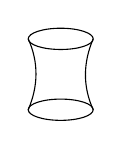
\begin{tikzpicture}[scale=0.75]
\draw (0,1.2) ellipse (0.55 and 0.18);
\draw (0,0) ellipse (0.55 and 0.18);
\draw (-0.55,1.2) .. controls (-0.37,0.80) and (-0.38,0.40) .. (-0.55,0);
\draw (0.55,1.2) .. controls (0.38,0.80) and (0.37,0.40) .. (0.55,0);
\end{tikzpicture}
\end{adjustbox}
\end{center}
Индекс пересеч.
\Unclear{GELFAND-P000492}{intersection-cancellation}{[Зачёркнуто: неразборчиво.]}
вещ. гомол. средней разм. (целочисл.)

Она знакоопр. [вставлено: (отр. опр.)] в точности в перечисл. случаях,
если только $n\equiv3\ (\mathrm{mod}\ 4)$.
(иначе доб. лишние перем.) --- теор. Тюрина.
\begin{equation*}
f^{-1}(\varepsilon)\cap B_\delta\approx
\underbrace{S^{n-1}\vee\ldots\vee S^{n-1}}_{\mu}.
\end{equation*}
$\mu=\dim$ лок. кольца.

\begin{center}
\begin{adjustbox}{max width=\linewidth}
\begin{tikzpicture}[scale=0.85]
\draw (0,0)--(3.2,0);
\draw (1.6,0)--(1.6,-0.55);
\draw (0,0) circle (0.04);
\fill (0.8,0) circle (0.04);
\draw (1.6,0) circle (0.04);
\draw (2.4,0) circle (0.04);
\draw (3.2,0) circle (0.04);
\draw (1.6,-0.55) circle (0.04);
\node at (0,0.32) {$-2$};
\node at (0.40,-0.30) {$1$};
\node at (4.30,0) {$E_6$};
\end{tikzpicture}
\end{adjustbox}
\end{center}
\Unclear{GELFAND-P000492}{graph-cancellation}{[Справа от $E_6$ зачёркнута короткая неразборчивая запись.]}

Кв. форма зад. сх. Дынкина.

\fbox{$m=1$.} --- тоже находится список (длинный).

Первая: $\underline{x_1^3+x_2^3+x_3^3}$.
\begin{equation*}
\underline{\mu=\mu_++\mu_0+\mu_-}
\end{equation*}
\begin{equation*}
\underline{\mu_+\le1}\quad\Rightarrow\quad\text{всегда }m=1.
\end{equation*}
\Unclear{GELFAND-P000492}{modality-inequality}{Знак перед $1$ усилен несколькими штрихами; дано чтение $\le$. В заключении написано $m=1$.}
У них у всех
\begin{equation*}
\mu_+\le1\Rightarrow\mu_0=1\qquad(\text{всегда вырожд.})
\end{equation*}
\underline{$\mu_+=1$.}\quad
$axyz+x^k+y^\ell+z^m$ --- \underline{3-х инд. серии} $T_{k\ell m}$.

\underline{А.С. Мищенко.}

\underline{Сулливан:} локализация, периодичн. и \ldots\ Галуа-
\begin{equation*}
K(X)/\text{$J$-эквив.}=J(X)\quad\text{--- \underline{конечн. группа}}.
\end{equation*}
Адамс: она опис. в терм. когом. опер. $K$-теории $\psi^k$.
\begin{equation*}
\psi^k(\xi)=\xi^k\quad\text{и \underline{аддитивны}}
\quad\Rightarrow\quad\text{этим они однозн. опред.}
\end{equation*}
$(\dim\xi=1)$\qquad $k=2,3,\ldots$

Итак $J(X)$ опр. группой $K(X)$ как модулем над этими опер.

$J$-экв. --- послойная гомот. экв.
\begin{equation*}
\begin{adjustbox}{max width=\linewidth}
\begin{tikzcd}[row sep=small,column sep=small]
\xi \arrow[rr,"f"] \arrow[dr] && \eta \arrow[dl]\\
& X &
\end{tikzcd}
\end{adjustbox}
\end{equation*}
$f$ --- собств.\quad $\operatorname{deg} f=1$ в слоях.

Было док. (Адамс, Атья):
$\xi\overset{J}{\sim}$ трив.

$X$ --- конечн. комплекс.
[Вставлено: тогда $\exists N\in Z$:]
$\forall$ $J$-трив. рассл. $\xi$
[вставлено: $\forall k$]
$\exists$
\Unclear{GELFAND-P000492}{bundle-cancellation}{[Зачёркнутое слово перед «рассл.» неразборчиво.]}
рассл. $y$:
\Unclear{GELFAND-P000492}{formula-cancellation}{[После двоеточия зачёркнут небольшой неразборчивый фрагмент.]}
\begin{equation*}
\underline{\xi=k^N(\psi^k-1)y}
\end{equation*}
\underline{Обратное --- гипотеза Адамса:}
$\forall$ кон. компл. $X$ $\exists N$; $\forall k$
\begin{equation*}
k^N(\psi^k-1)\xi\overset{J}{\sim}0.
\end{equation*}

\SourcePage{GELFAND-P000493}{unlabelled}
\underline{Идея.}
\begin{equation*}
\begin{adjustbox}{max width=\linewidth}
\begin{tikzcd}[column sep=large]
\xi=f^*(\xi) \arrow[d] & \xi_n \arrow[d]\\
X \arrow[r,"f"] & BU(n)=G_{n,\infty}
\end{tikzcd}
\end{adjustbox}
\end{equation*}
\begin{equation*}
\begin{adjustbox}{max width=\linewidth}
\begin{tikzcd}[column sep=large]
f^*(\eta) \arrow[d] & \eta \arrow[d]\\
X \arrow[r] & Y
\end{tikzcd}
\end{adjustbox}
\end{equation*}
\begin{equation*}
\psi^k(f^*(\eta))=f^*\psi^k(\eta).
\end{equation*}
Отсюда опер. $\psi^k$ опр. заданием рассл. на \underline{$BU(n)$}.
$(\psi^k(\xi_n))$.

По $\psi^k$ строится отобр.
$BU(n)\longrightarrow BU(\infty)$ (неизв. размерность).

$\psi^k(1)=1\Rightarrow$ получ., что $\exists$ послед. отобр.
\begin{equation*}
\begin{adjustbox}{max width=\linewidth}
\begin{tikzcd}[column sep=small]
\begin{gathered}\xi_n+1\\BU(n)\end{gathered}
\arrow[rr,"\psi^k"] \arrow[dr,swap,"\text{станд.}"] && BU(\infty)\\
& BU(n+1) \arrow[ur,swap,"\psi^k"] &
\end{tikzcd}
\end{adjustbox}
\end{equation*}
Итак, $\psi^k$ зад. одним отобр.
\begin{equation*}
\underline{BU(\infty)\overset{\psi^k}{\longrightarrow}BU(\infty)}.
\end{equation*}
\underline{Пусть есть когом. опер.}
$BU(\infty)\overset{A}{\longrightarrow}BU(\infty)$,
и пусть она сохр. разм.
\begin{equation*}
\begin{adjustbox}{max width=\linewidth}
\begin{tikzcd}[column sep=large]
BU(n) \arrow[r,"A"] \arrow[d] & BU(n) \arrow[d]\\
BU(\infty) \arrow[r,"A"] & BU(\infty)
\end{tikzcd}
\end{adjustbox}
\end{equation*}
[Справа:]
\underline{сохр. размерность.}
\underline{Их не бывает, но если бы они были, то можно было бы док., что}
$A\xi\overset{J}{\sim}\xi$.

Тогда $\underline{A\xi\overset{J}{\sim}\xi}$.

\fbox{сферы}
\begin{equation*}
\begin{adjustbox}{max width=\linewidth}
\begin{tikzcd}[column sep=large,row sep=large]
S(\xi_{n+1}) \arrow[r,"\sim","\text{гом. экв.}"'] \arrow[d] &
BU(n) \arrow[r,"A"] \arrow[d] & BU(n) \arrow[d] &
S(\xi_{n+1}) \arrow[l,swap,"\sim"] \arrow[d]\\
B(n+1) \arrow[r,equal] & BU(n+1) \arrow[r,"A"] \arrow[d] &
BU(n+1) \arrow[r,equal] \arrow[d] & BU(n+1)\\
& \vdots & \vdots &
\end{tikzcd}
\end{adjustbox}
\end{equation*}
\Unclear{GELFAND-P000493}{left-base-notation}{В левом нижнем узле написано $B(n+1)$, без $U$; обозначение сохранено.}

Получ. послойная гомот. эквив.

[Зачёркнуто: Но: как их]

Их нет, но как же их «найти»?
\begin{equation*}
\begin{adjustbox}{max width=\linewidth}
\begin{tikzcd}[column sep=large,row sep=small]
X \arrow[r,shift left=0.5ex] \arrow[r,shift right=0.5ex] &
BU(n) \arrow[rr,"J"] \arrow[dr] && B_F\\
&& BU(n)^{\wedge} \arrow[ur] &
\end{tikzcd}
\end{adjustbox}
\end{equation*}
(\underline{классиф. пр-во рассл. со слоем [вставлено: гомотоп.] сфера})

$J$ --- функтор.

Пусть $\exists BU(n)^{\wedge}$, на к-рое перен. операции Адамса,
т.е. $\exists$ опер. $(\psi^k)^{\wedge}$,
для к-рых коммут. диагр.
\begin{equation*}
\begin{adjustbox}{max width=\linewidth}
\begin{tikzcd}[column sep=large,row sep=large]
BU(n) \arrow[r] \arrow[d,swap,"\psi^k"] &
BU(n)^{\wedge} \arrow[r] \arrow[d,"(\psi^k)^{\wedge}"] & B_F\\
BU(\infty) \arrow[r] & BU(\infty) \arrow[ur,bend right=15] &
\end{tikzcd}
\end{adjustbox}
\end{equation*}
Быть может, может быть, что $(\psi^k)^{\wedge}$
\underline{сохр. размерность.}

(\underline{ориентации} --- сохр. разм. отобр.)

Эти пр-ва постр. Сулливаном.

\SourcePage{GELFAND-P000494}{unlabelled}
$BU(n)^{\wedge}$ будет пополн. грассман.

На \Unclear{GELFAND-P000494}{initial-cancellation}{[Зачёркнуто: неразборчиво.]}
\underline{$S^{2n-1}$ гр. $U(n)$}.
\Unclear{GELFAND-P000494}{sphere-exponent}{Знак в показателе $2n-1$ затушёван: $2n-1$ или $2n+1$.}
Получ. расслоение (сфер). на $BU(n)$.

\underline{Сулливан:} другое пр-во $\widehat S^{2n-1}$ и гр. $G_n$.
Рассм. рассл. и классиф. пр-во.
\begin{equation*}
\begin{adjustbox}{max width=\linewidth}
\begin{tikzcd}[column sep=large,row sep=large]
BU(n)^{\wedge} \arrow[r] \arrow[d] & BU(n+1)^{\wedge}\\
BU(n)^{\wedge} &
\end{tikzcd}
\end{adjustbox}
\qquad\widehat S^{2n+1}
\end{equation*}
и будет сохр. послойный гомот. тип.

\Incomplete{GELFAND-P000494}{obliterated-line}{[Зачёркнутая строка перед «Рассматриваются односвязные компл.» не поддаётся связному чтению; её словесное содержание не восстановлено.]}

Рассматриваются односвязные компл. с кон. порожд. гомот. гр.

\underline{Утв.} [Вставлено: $\forall X$] $\exists$
\begin{equation*}
\begin{adjustbox}{max width=\linewidth}
\begin{tikzcd}[column sep=small,row sep=large]
X \arrow[rr,"\alpha(X)"] \arrow[dr,swap,"\forall f"] &&
\widehat X \arrow[dl,"\widehat f\ (\exists\text{ и ед.})"]\\
& F &
\end{tikzcd}
\end{adjustbox}
\end{equation*}
(функтор)

$\alpha(X)$ --- преобр. тожд. функтора.

$(\forall F,$ [вставлено: у к-ро] $\pi_i(F)$
\Unclear{GELFAND-P000494}{finite-cancellation}{[Затушёванный фрагмент перед «конечны» неразборчив.]}
конечны$)$.

\underline{$\pi_i(\widehat X)$ проконечны}
($\underset{\longleftarrow}{\lim}$ кон. групп).
(в частн., компактны).

\Unclear{GELFAND-P000494}{before-then-cancellation}{[Зачёркнуто: «В частности»?]}
Тогда можно выч.:
\begin{equation*}
\pi_i(\widehat X)=\widehat{\pi_i(X)}
\end{equation*}
(прокон. пополнение).
Окр. --- подгруппы кон. индекса и их предел.

$Z^{\wedge}$ опис. через [вставлено: целые] $p$-адич. числа.

Гом. группы $\widehat X$ ведут себя как целые $p$-ад. числа.

[Зачёркнуто: Действие гр. Галуа.]
\begin{equation*}
\begin{adjustbox}{max width=\linewidth}
\begin{tikzcd}[column sep=large,row sep=large]
BU(n) \arrow[r] \arrow[d] & \widehat{BU(n)} \arrow[d]\\
B_F \arrow[r,"="] & \widehat B_F
\end{tikzcd}
\end{adjustbox}
\end{equation*}
[К $B_F$:] все гом. гр. конечны (это стаб. гомот. группы сфер).

\SourceFigure{GELFAND-P000494}{lower-completion-diagram}{Схема с цепочками $S^{2n+1}\to BU(n)\to BU(n+1)$ и $\widehat S^{2n+1}\to\widehat{BU(n)}\to\widehat{BU(n+1)}$, горизонтальными связями между $BU(n)$ и $\widehat{BU(n)}$, между нижними основаниями, а также стрелкой из $\widehat{BU(n)}$ к $B_F$. Требуется проверить левый конец нижней горизонтальной стрелки и точное наложение верхней правой стрелки на соседнюю надпись.}

[Зачёркнуто: Пусть]
\Unclear{GELFAND-P000494}{adams-cancellation}{[Следующее короткое зачёркнутое слово неразборчиво.]}
[Вставлено: Постр. опер.
\Unclear{GELFAND-P000494}{adams-operation-index}{$\psi_k$ или $\widehat\psi^k$?}]
прод. опер. Адамса и сохр. размерность.

Рассм. грассманы: $G_{N,n}$.
Это конечн. число афф. алг. карт, где ур-я над $Z$ (сх. над $Z$).
--- алг. мн-зие над $Q$.
$\Rightarrow$ там действ. гр. Галуа $\operatorname{Gal}(C:Q)$
--- действует на $G_{N,n}$.
Оно не непр. в об. смысле, но непр. в топ. Зарисского.
Рассм. \underline{Étale-топ.} \ldots
\begin{equation*}
\operatorname{Gal}(C:Q)\longrightarrow
\operatorname{Gal}(Q_{ab};Q)=\widehat Z^{*}
\end{equation*}
[Под $Q_{ab}$: max аб. расш.]
\begin{equation*}
H_i(V_c,A)\approx H_i(V_{et},A)
\end{equation*}
\begin{equation*}
\widehat V_c\sim\underset{\longleftarrow}{\lim}\,N(V_{et}),
\qquad N\text{ --- нерв.}
\end{equation*}

\SourcePage{GELFAND-P000495}{unlabelled}
\underline{26.3.73}

\underline{Формулир. рез. Атья, Патоди, Зингер. (И.М. Гельфанд).}

Пусть $A$ --- самосопр. элл. опер.
\begin{equation*}
\zeta_A(s)=\operatorname{Tr}A^{-s}=\sum\lambda_i^{-s}
\end{equation*}
при $s=0$ не имеет полюса (Сили).

$\zeta_A(0)$ --- Атья и другие.

Рассм. вместо $\zeta$-ф-и $L$-ряды.
\Incomplete{GELFAND-P000495}{eta-cancelled-phrase}{[Справа после «$L$-ряды» зачёркнута фраза; кроме возможного начального «Не» её текст не восстановлен.]}
[Справа: \underline{Пусть $A$ --- не полож. опред.} (самосопр. эллипт.)]
\begin{equation*}
\eta(s)=\sum_{\lambda\ne0}(\operatorname{sign}\lambda_i)\,|\lambda_i|^{-s}
\end{equation*}
Трудная теор.: \underline{$s=0$ --- не полюс} !!

Сущ. пример --- опр. 1-го порядка.

Общая зад.: нет полож. опред. Рассм. $\sum$ (мульт. характеров от $\lambda_i$)
($L$-ряды).
\underline{На компл. числах быв. более сложные мульт. характеры.}

\underline{Пример.}
\Unclear{GELFAND-P000495}{example-cancellation}{[Перед $A$ и частично поверх него затушёванный знак; неразборчиво.]}
\begin{equation*}
A=i\frac{d}{dx}+t\qquad\text{на }[0,2\pi]\qquad\text{периодич.}
\end{equation*}
\begin{equation*}
\underline{\eta(0)=1-2t}
\end{equation*}
\Unclear{GELFAND-P000495}{eta-value-domain}{[Видимая формула: $\eta(0)=1-2t$; область значений $t$ здесь не указана.]}

Соб. знач. $n+t$, $n=-2,-1,0,1,\ldots$

$\eta(0)$ --- «асимметрия» оператора:
\begin{equation*}
\sum_{\lambda_i>0}1-\sum_{\lambda_i<0}1.
\end{equation*}

\underline{С.И. Гельфанд.} Излож. последней лекции Манина:

$p$-адич. интегрирование (Мазур,
\Unclear{GELFAND-P000495}{swinnerton-spelling}{Суиннертон --- Дайер?})

\SourcePage{GELFAND-P000496}{unlabelled}
$Z_p$ --- целые $p$-адич. числа, на них задана ф-я. Надо проинтегрировать.

(знач. $p$-адические)

\underline{лит.} Л.Г. Шнирельман, Дворк, Грауэрт, Краснер, Тэйт

$Z_p\supset A_i=p^iZ_p$ --- сист. окр. $0$.
Мера зад. на мн-вах $a+A_i$.

$\mu(a+A_i)$ --- $p$-адич. число (не обяз. целое).

$a\in Z_p$ или \underline{$a\in Z_p/p^i$}.

Должна быть конечн. аддитивность; свод. к усл.:
\begin{equation*}
\mu(a+A_i)=\sum_{t=0}^{p-1}\mu(a+tp^i+A_{i+1})
\end{equation*}

\underline{2 примера:} 1) \underline{инвар. мера}: не зав. от $a$, а зав. от $i$. Тогда
\begin{equation*}
\mu(a+A_i)=p^{-i}\qquad\text{(единств. возможность).}
\end{equation*}
Мера мал. мн-ва велика! --- далеко от $0$
\begin{equation*}
\left(\left\|\frac ab\right\|=p^{-n},\quad
\text{где }\frac ab=p^n\frac{a_1}{b_1},\quad
 a_1,b_1\text{ вз. пр. с }p\right).
\end{equation*}

2) \underline{Более важный пример.} (меры Леопольда--Куботы).
[Справа: 2 параметра $n$ и $a$]
\begin{equation*}
(n,p)=1,\qquad 0\le a\le p^i-1
\end{equation*}
\begin{equation*}
\mu_n(a+A_i)=\left[\frac{na}{p^i}\right]-\frac{n-1}{2}
\end{equation*}
\begin{equation*}
\mu_2(a+A_i)=
\begin{cases}
+1/2,\text{ если }a>\dfrac{p^i}{2},\\
-1/2,\text{ если }a<\dfrac{p^i}{2}.
\end{cases}
\end{equation*}
Она аддит. !! Мера $\forall$ мн-ва ограничена

(она получ. преобр. Меллина из $\zeta$-ф-и Леопольда--Ивасавы)

$Q_p\ni f(x)$, $x\in Z_p$
\begin{equation*}
\int_{Z_p}f(x)\mu(x)\qquad\text{по Риману}
\end{equation*}
$R_m$ --- представители $Z_p/p^mZ_p$ (по 1 из $\forall$ класса).

Это разбиение. Сост.
\begin{equation*}
S(R_m)=\sum_{a\in R_m}f(a)\mu(a+A_m)
\end{equation*}
они сходятся при усл. на меру и ф-ю.

\underline{Умеренно раст. мера} --- если растёт медленнее инвариантной
\begin{equation*}
\lim_{m\to\infty}\max|\mu(a+A_m)|p^{-m}=0
\end{equation*}
$f$ уд. усл. Липшица, если
$|f(a)-f(b)|<Cp^{-m}$, если $|b-a|<p^{-m}$

(в частн., если зад. сход. степ. рядом)

Если мера умер. растёт, а ф-я удовл. усл. Липшица, то $\exists$ предел, наз. интегралом.

\SourcePage{GELFAND-P000497}{unlabelled}
Если рассм. обычную $\zeta(s)=\sum1/n^s$. Тогда

$\zeta(1-2k)$ --- рац. число $\forall k>0$ (выр. через Берн. числа).

\Unclear{GELFAND-P000497}{margin-cancellation}{[На левом поле зачёркнутый математический знак или короткое выражение; неразборчиво.]}
Пусть $k_i$ --- [зачёркнуто: $p$-адич. числа] целые и в $p$-ад. смысле
\begin{equation*}
k_i\longrightarrow a\in Z_p.
\end{equation*}
\underline{Ивасава--Леопольд:}
\begin{equation*}
\underline{\zeta(1-2k_i)\overset{p}{\longrightarrow}\zeta(a)}\quad!!
\end{equation*}
\Unclear{GELFAND-P000497}{zeta-limit-formulation}{[Предел записан с $\zeta(a)$ справа; дополнительные условия на последовательность и нормировка здесь не приведены.]}

Получ. непр. ф-я на $Z_p$ ---
\Unclear{GELFAND-P000497}{variable-cancellation}{[Короткое зачёркнутое слово неразборчиво.]}
$p$-адич. перем. Она есть преобр. Меллина меры примера 2.

\underline{А. Габриэлов.} \underline{Диагр. Дынкина изол. особ. ф-й.}

$f(x)$ --- компл.-аналит. в окр. $0$, $0$ --- изолир. особ.

Шар рад. $r_0$ (малое). Рассм.
\begin{equation*}
\underline{f(x)=\delta,\quad |x|<r_0}
\end{equation*}
[Вставлено: \underline{Выб. ещё $\delta$.}]

При малом $\delta$ это компл. мн-зие разм. $(n-1)$, гомот. экв. букету
\Unclear{GELFAND-P000497}{sphere-dimension}{$(n-1)$ или $(k-1)$?}-сфер.

и исчез. циклы.

\SourcePage{GELFAND-P000498}{unlabelled}
\underline{9/IV-73 г.}
\Unclear{GELFAND-P000498}{header-cancellation}{[Справа от даты зачёркнуто короткое слово: «Сем.»?]}

\underline{С.И. Гельфанд.} (излож. лекций Ю.И. Манина)

$Q_p\supset Z_p$,

\{Мера $\mu$ на $Z_p$ со знач. в кон.-мерном пр-ве $W$ над $Q_p$.\}
\begin{equation*}
\mu:U\longmapsto\mu(U)\in W,\qquad U\subset Z_p
\end{equation*}
\begin{equation*}
\mu(U_1\cup U_2)=\mu(U_1)+\mu(U_2).
\end{equation*}
\Unclear{GELFAND-P000498}{additivity-condition}{[Условие непересечения $U_1$ и $U_2$ при этой формуле не написано.]}

В $Q_p$ базис откр.-замкн. мн-в $A_n=p^nZ_p$.
$U=(a+A_n)$.

Интеграл по Риману.

$f$ --- ф-я на $Z_p$ со знач. в $Q_p$.

$m\ge1$,

$R_m$ --- представители $Z_p/p^mZ_p$. (конечное мн-во).

Сумма Римана
\begin{equation*}
S(R_m)=\sum_{a\in R_m}f(a)(a+A_m)
\end{equation*}
\Unclear{GELFAND-P000498}{riemann-missing-mu}{[В записанной сумме перед $(a+A_m)$ знак $\mu$ отсутствует.]}

\underline{Теор.:} при $m\to\infty$ при нек-рых усл. на ф-ю и меру $\exists$ предел
\begin{equation*}
\lim_{m\to\infty}S(R_m)=\int_{Z_p}f(a)\mu(a)\in W
\end{equation*}
\underline{Условия:} $\mu$ ограничена, а ф-я лок. постоянна

\underline{меры Леопольда--Куботы:}

$k$ --- целое, $(k,p)=1$,
\begin{equation*}
\mu_k(a+A_n)=\left[\frac{ka}{p^n}\right]-\frac{k-1}{2}
\end{equation*}
$0\le a\le p^n-1$

Легко пров. (полезно), что она конечно-аддит.

(Преобр. Меллина [Вставлено в выноске: Этой меры --- $\zeta$-ф-я]
мульт. $p$-адич. хар. на $Z_p$)

Мульт. хар.: $p$-адич. число в $p$-адич. степени.
\begin{equation*}
\chi_t(a)=e^{t\ln a},\qquad a=1\bmod p.
\end{equation*}
\Unclear{GELFAND-P000498}{t-cancellation}{[Зачёркнуто условие, начинающееся с $t$; следующие знаки неразборчивы.]}
\underline{$t\in Z_p$} (чтобы сходилось)
\begin{equation*}
\ln a=(a-1)-\frac{(a-1)^2}{2}+\ldots
\end{equation*}
\Unclear{GELFAND-P000498}{log-denominator}{[В знаменателе видна $2$ под затушёванными штрихами; прежний знак не восстановлен.]}

\underline{2-й кл. мер с пом. модулярных форм:}
\begin{equation*}
H=(z\mid\operatorname{Im}z>0)
\end{equation*}
Действ.
\begin{equation*}
SL(2,R)/(\pm1)\supset\Gamma=SL(2,Z)/(\pm1)
\end{equation*}
Рассм.
\begin{equation*}
\varphi(z)=\sum_{n=1}^{\infty}\lambda_n e^{2\pi inz}
\qquad\text{(различ. инвар. убыв. ф-и)}
\end{equation*}
Автом. форма веса $w$
\begin{equation*}
\varphi(gz)=(az+c)^{-w}\varphi(z),\qquad
 g=\begin{pmatrix}a&b\\c&d\end{pmatrix},\quad g\in\Gamma.
\end{equation*}
\Unclear{GELFAND-P000498}{automorphy-factor}{[В множителе написано $(az+c)^{-w}$; буквы $a$ и $c$ сохранены.]}
% GELFAND-0052. Diplomatic transcription; no catalogue heading is supplied as handwriting.
% Editorial descriptions are in Russian square brackets. The source remains authoritative.
% Coordinates below are original PNG pixels: (left, top, right, bottom), half-open,
% origin at upper left; both frames are 2415 x 3480. Enlargement adds no source pixels.
\SourcePage{GELFAND-P000499}{unlabelled}
% One visible portrait leaf; no confidently readable label, date, or speaker heading.
% Review: top (180,35,1390,190), 3x; sum (385,185,1250,485), 3x;
% summand glyph (920,195,991,290), 10x; eigenvalue lines (275,495,2015,812), 3x.

Ещё условие: $\varphi$ \underline{\underline{собств.}} отн.
[Вставлено над строкой и обведено: всех] операторов Гекке.
\begin{equation*}
(T_k\varphi)(z)=\sum_{\substack{ad=k\\0\le b\le d-1}}
f\left(\frac{az+b}{d}\right)
\end{equation*}
\Unclear{GELFAND-P000499}{hecke-summand}{$f$ [так в рукописи; слева $\varphi$].}
\begin{equation*}
(a,b,d,k\text{ — целые})
\end{equation*}
$T_k\varphi$ — тоже модулярн. форма

Пусть $\lambda_1=1$. Тогда
\begin{equation*}
T_k\varphi=\lambda_k\varphi
\qquad(\lambda_k\text{ — коэфф. при }e^{2\pi ikz}).
\end{equation*}
\begin{center}\rule{1.4cm}{0.3pt}\quad\rule{1.6cm}{0.3pt}\end{center}

% Review: character (240,825,1770,1100), 3x;
% exponent (650,997,795,1051), 10x; obscured sign (724,1008,765,1032).
\begin{equation*}
p:\qquad\chi:(\mathbb{Z}/p^n\mathbb{Z})^*\to\mathbb{C}^*
\end{equation*}
(примитивный характер)\qquad($p^n$ — кондуктор хар.)
\begin{equation*}
(\text{на }p^{n\,\text{[неясный знак]}\,1}\mathbb{Z}/p^n\mathbb{Z}\text{ нетрив.})
\end{equation*}
\Unclear{GELFAND-P000499}{primitive-exponent}{Показатель степени: $n-1$ или $n+1$.}

% Review: twist (270,1125,1635,1265), 3x;
% overwritten multiplier (746,1284,824,1386), 10x;
% Mellin formula (405,1450,2070,1655), 3x; capital Phi glyphs (439,1510,986,1619), 5x.
% Separator dot below: (800,1685,1350,1745), 5x.
\begin{equation*}
\varphi_\chi(z)=\sum\lambda_n\chi(n)e^{2\pi inz}
\quad\text{— тоже модулярн.}
\end{equation*}
\begin{equation*}
L(\varphi,\chi,1)=\text{[густо переписанный множитель]}
\int_0^{i\infty}\varphi_\chi(z)\,dz
\end{equation*}
\Unclear{GELFAND-P000499}{l-one-prefactor}{$C$? [Видны также неразборчивые наложенные штрихи.]}

Имеет интерпретацию
\begin{equation*}
L(\Phi,\chi,s)=C\int_0^{i\infty}\Phi_\chi(z)z^{s-1}\,dz
=\sum\frac{\lambda_n\chi(n)}{n^s}\qquad(L\text{-ф-я})
\end{equation*}
\begin{center}\rule{2cm}{0.3pt}\quad$\cdot$\quad\rule{2.3cm}{0.3pt}\end{center}

% Review: p-adic text (270,1735,1880,1940), 3x; target (200,1930,2100,2305), 3x;
% circled question mark (930,2150,1025,2255), 8x. The question mark is source ink.
% Separator dot below: (870,2265,1135,2325), 5x.
$p$-адич. часть.

$\chi$ — также лок. пост. ф-я на целых $p$-адич. числах

(на обрат. — так, а дальше $0$).

Пусть $\chi(-1)=1$

Цель: $L(\varphi,\chi,1)$ предст. через $\int\chi$ на $p$-адич. числах.
\begin{equation*}
\int\chi(a)\mu(a)=\text{[обведён знак вопроса: ?]}L(\varphi,\chi,1).
\end{equation*}
\begin{center}\rule{1.2cm}{0.3pt}\quad$\cdot$\quad\rule{1cm}{0.3pt}\end{center}

% Review: path and surrounding text (260,2290,1310,2615), 3x;
% full path context (300,2140,1850,2595), 3x; final abbreviation (1190,2520,1720,2640), 5x.
% Conservative diagram: horizontal baseline, vertical paths at 0 and x,
% wavy joining top, no arrows or interior labels. Integral at left, annotation at right.
\begin{center}
$\displaystyle\int_0^x\varphi(z)\,dz$
\quad
\begin{adjustbox}{max width=\linewidth}
\begin{tikzpicture}[baseline=0pt]
\draw (-0.5,0)--(2.9,0);
\draw (0,0)--(0,1.25)
.. controls (-0.05,1.5) and (0.25,1.58) .. (0.6,1.47)
.. controls (0.95,1.38) and (1.1,1.59) .. (1.35,1.48)
.. controls (1.65,1.38) and (1.95,1.7) .. (2.25,1.51)
.. controls (2.47,1.37) and (2.31,1.2) .. (2.4,1.05)
--(2.4,0);
\node[below] at (0,0) {$0$};
\node[below] at (2.4,0) {$x$};
\end{tikzpicture}
\end{adjustbox}
\quad\underline{$x$ — рац. точка.}
\end{center}

(по существу $\int$ по циклу на факторпр-ве)

% Review: period and algebraic text (85,2580,1930,2880), 3x;
% ell (96,2617,207,2733), 10x; adjective (735,2630,1110,2750), 5x;
% right annotation (1330,2600,1980,2800), 3x.
\begin{equation*}
\ell(x)=\frac{1}{\omega}\operatorname{Re}\int_0^x\Phi(z)\,dz
\text{ — целое алг.}
\end{equation*}
из фикс. расш. $Q$.

[Справа: $\exists\omega$ (трансценд.)]

(во многих случаях)

% Review: roots and limit (360,2890,2110,3230), 3x; w (817,2886,931,2952), 10x;
% denominator (1140,3060,1367,3142), 10x; limit (946,3138,1078,3212), 8x;
% congruence/residue (1390,3178,1510,3246), 10x; summation indices (1365,3120,1630,3240), 8x.
\begin{equation*}
T^2-\lambda_pT+p^{w-1}=0,\qquad
\pi,\bar\pi\text{ — корни},\qquad\lambda_p\ne0\bmod p.
\end{equation*}
\begin{equation*}
\mu(a+A_n)=\lim_{\substack{m\to\infty\\m\ge n}}
\frac{1}{\pi^m+\bar\pi^m}
\sum_{\substack{b\bmod p^m\\b\equiv\text{[неясно]}\bmod p^n}}
\ell\left(\frac{b}{p^m}\right)
\end{equation*}
\Unclear{GELFAND-P000499}{measure-residue}{Остаток после $\equiv$: $a$ или $0$.}

$\lim$ сущ.

Оконч. результат:
% Review: final line (280,3190,1950,3460), 3x;
% exponent k (949,3270,1110,3365), 10x; g (1465,3360,1645,3437), 10x.
\begin{equation*}
\pi^{k-1}\int_{\mathbb{Z}_p}\chi^{-1}(a)\mu(a)
=-\frac{p^k}{\omega g(\chi)}L(\Phi,\chi,1)
\end{equation*}

\SourcePage{GELFAND-P000500}{unlabelled}
% One visible portrait leaf. The ambiguous right-margin mark is recorded below.
% Review: heading (175,40,840,155), 4x; cancelled word (184,65,365,120), 8x;
% first equation (310,160,1565,281), 3x; Taylor lines (370,290,1680,895), 3x.

[Зачёркнуто: \Unclear{GELFAND-P000500}{top-cancelled-word}{Числа?}]
\underline{И. М. Гельфанд.}
[Под именем — полоса между двумя чертами с поперечной штриховкой.]

\begin{gather*}
1^k+2^k+\ldots+n^k=P_{k+1}(n)\quad\text{— \underline{полином Бернулли.}}\\
\sum_{i=1}^{n}f(i),\qquad F'(x)=f(x).
\end{gather*}
\begin{align*}
F(n+1)-F(n)&=f(n)+\frac{f'(n)}{2!}+\frac{f''(n)}{3!}+\ldots\\
F(n)-F(n-1)&=f(n-1)+\frac{f'(n-1)}{2!}+\frac{f''(n-1)}{3!}+\ldots\\[1em]
F(2)-F(1)&=f(1)+\frac{f'(1)}{2!}+\ldots
\end{align*}
% Review: margin mark (1795,750,1915,855), 8x.
[Справа: \Unclear{GELFAND-P000500}{right-margin-mark}{36 / 38? [Густо наведённый знак с коротким штрихом ниже слева.]}.]

% Review: middle equations and sums (265,923,2140,1600), 3x;
% right definitions (1680,915,2185,1380), 3x.
Отсюда
\begin{equation*}
F(n+1)-F(1)=S_n+\frac{S'_n}{2!}+\frac{S''_n}{3!}+\ldots
\end{equation*}
[Справа, за двойной вертикальной чертой:]
\begin{gather*}
S_n=\sum_{i=1}^{n}f(i)\\
S'_n=\sum_{i=1}^{n}f'(i)\\
\ldots\qquad\ldots\qquad\ldots\\
S_n^{(k)}=\sum_{i=1}^{n}f^{(k)}(i)
\end{gather*}

Аналогично:
% Review: entire cancellation (250,1115,1140,1250), 4x;
% left part (505,1155,817,1240), 8x; right part (805,1145,1120,1227), 8x.
[Зачёркнуто:
\Unclear{GELFAND-P000500}{middle-cancelled-phrase}{И? возьмем? [далее скрытый текст] $S_i$ или $\Sigma_i$}.
\Incomplete{GELFAND-P000500}{middle-cancelled-gap}{Слова между предполагаемым «возьмем» и последним знаком закрыты густыми зачёркиваниями и не восстановлены.}]
\begin{align*}
f(n+1)-f(1)&=S'_n+\frac{S''_n}{2!}+\ldots\\
f'(n+1)-f'(1)&=S''_n+\ldots
\end{align*}
Будем рассм. это как сист. ур-й относит. $S_n,S'_n,S''_n,\ldots$

Отсюда
% Review: determinant (305,1580,1690,2015), 3x and (515,1560,1715,2050), 3x.
% Exactly three written rows; first-row fractions stacked, later fractions with slashes.
% Descending points at the right and the blank lower extension of the bars are retained.
\begin{equation*}
S_n=\begin{vmatrix}
F(n+1)-F(1)&\dfrac{1}{2!}&\dfrac{1}{3!}&\dfrac{1}{4!}&\\
f(n+1)-f(1)&1&1/2!&1/3!&\vdots\\
f'(n+1)-f'(1)&0&1&1/2!&\\
&&&&
\end{vmatrix}=
\end{equation*}

Раскроем по 1-му столбцу:
% Review: expansion (310,2040,2165,2425), 3x; B2 primes (1560,2170,2025,2305), 8x.
\begin{equation*}
=B_0\bigl(F(n+1)-F(1)\bigr)+B_1\bigl(f(n+1)-f(1)\bigr)+B_2\bigl(f'(n+1)-f'(1)\bigr)+\ldots
\end{equation*}
Но: $B$ не зависят от вида ф-и!

% Review: exponential example (280,2400,2180,2780), 3x;
% cancelled sum (292,2575,470,2660), 10x.
Возьмём $f(x)=e^{tx}$. Тогда $f'(x)=te^{tx}$.
[Справа: Геом. прогр.]

[Слева зачёркнуто: $\sum$
\Incomplete{GELFAND-P000500}{lower-cancelled-sum}{Продолжение выражения и возможные индексы знака суммы скрыты густыми штрихами; не восстановлены.}]
\begin{equation*}
\underline{S_n=\frac{e^{t(n+1)}-e^t}{e^t-1}}
\end{equation*}
\underline{разлагаем по $t$}

[Подчёркнуто волнистой линией: в степ. ряд — получим коэффициенты.]

% Review: final Russian line (355,2780,1790,2880), 4x;
% upper bibliography (285,2910,2370,3177), 3x; lower bibliography (305,3160,2415,3435), 3x;
% German title left (315,3260,1540,3390), 4x; right (1500,3250,2395,3410), 4x.
Числа Бернулли в любых полях.

\underline{\underline{Math. Z.}}, \underline{\underline{1898}} \underline{Гурвиц}
[Подчёркнуто волнистой линией: (Аналог чисел Бернулли для Гауссовых чисел)]

Hurwitz, Math. Ann., 1899, стр. 196–226

(\underline{Über die Entwicklungskoeffizienten der Lemniskatischen}
\newline
\underline{\Unclear{GELFAND-P000500}{german-final-word-case}{functionen / Functionen}}).

\end{document}
